


\newcommand{\papertitle}{Quantum Mechanics and Quantum Gravity in the Vortex Æther Model\\
{\large A Reformulation Using Superfluid Vorticity and Topology}}
\newcommand{\paperdoi}{10.5281/zenodo.15870861}


\documentclass[a4paper,12pt]{article}
\usepackage{../vamstyle}
\usepackage{setspace}

\usepackage{import}
\usepackage{subfiles}
\usepackage{amsmath,amssymb,amsfonts}
\usepackage{url}
\usepackage{textcomp}           % supports some symbols like ℓ
\usepackage[bottom,hang,multiple]{footmisc}


\renewcommand{\footnotelayout}{\tiny}
\usepackage{float}
\usepackage{booktabs}
\usepackage{caption}
\usepackage{newunicodechar}     % fix undefined unicode symbols
% Fix unicode issues
\newunicodechar{ℓ}{\ensuremath{\ell}}
\newunicodechar{π}{\ensuremath{\pi}}
\newunicodechar{τ}{\ensuremath{\tau}}
\newunicodechar{θ}{\ensuremath{\theta}}
\newunicodechar{₂}{\textsubscript{2}}
\newunicodechar{₃}{\textsubscript{3}}


% vamappendixsetup.sty

\newcommand{\titlepageOpen}{
  \begin{titlepage}
  \thispagestyle{empty}
  \centering
  {\Huge\bfseries \papertitle \par}
  \vspace{1cm}
  {\Large\itshape\textbf{Omar Iskandarani}\textsuperscript{\textbf{*}} \par}
  \vspace{0.5cm}
  {\large \today \par}
  \vspace{0.5cm}
}

% here comes abstract
\newcommand{\titlepageClose}{
  \vfill
  \null
  \begin{picture}(0,0)
  % Adjust position: (x,y) = (left, bottom)
  \put(-200,-40){  % Shift 75pt left, 40pt down
    \begin{minipage}[b]{0.7\textwidth}
    \footnotesize % One step bigger than \tiny
    \renewcommand{\arraystretch}{1.0}
    \noindent\rule{\textwidth}{0.4pt} \\[0.5em]  % ← horizontal line
    \textsuperscript{\textbf{*}}Independent Researcher, Groningen, The Netherlands \\
    Email: \texttt{info@omariskandarani.com} \\
    ORCID: \texttt{\href{https://orcid.org/0009-0006-1686-3961}{0009-0006-1686-3961}} \\
    DOI: \href{https://doi.org/\paperdoi}{\paperdoi} \\
    License: CC-BY 4.0 International \\
    \end{minipage}
  }
  \end{picture}
  \end{titlepage}
}
\begin{document}

    % === Title page ===
    \titlepageOpen


\begin{abstract}



            We present a unified reformulation of quantum mechanics and gravitation within the Vortex Æther Model (VAM) — a framework in which all known particles and fields emerge as topologically stable excitations in a compressible, inviscid superfluid medium. In this approach, wavefunctions correspond to rotating swirl-phase patterns of knotted vortices, and canonical commutation relations arise from the interplay between fluid density and circulation. We derive the Schrödinger equation from first principles as a nonlinear limit of æther-phase evolution, establish a fluid-dynamic analog of the uncertainty principle, and interpret spin-½ behavior as a topological phase acquired under 4π rotation of chiral knots.


            Gravitational effects emerge from pressure gradients and swirl-induced curvature in the æther, replacing spacetime curvature with vortex geometry. We demonstrate that black hole thermodynamics, including Hawking-like radiation and entropy bounds, follow from quantum-swirl phase quantization near vortex horizons. By introducing a layered time framework — combining background æther time, local swirl-clock phase, and discrete reconnection (Kairos) transitions — we account for entanglement, measurement collapse, and temporal asymmetry without invoking external observers.


            The VAM framework recovers key quantum-gravitational phenomena with minimal assumptions and a unified ontology. It suggests new directions for experimental testing in condensed matter systems, predicts the existence of chirality-constrained neutral particles, and proposes fluid-derived values for $\hbar$ and $G$. This work lays the foundation for a topological fluid model of quantum gravity that is both conceptually transparent and physically predictive.




\end{abstract}


\titlepageClose


\tableofcontents
\newpage

\section{Introduction and Motivation}
    Modern physics is built on two pillars that remain deeply incompatible: quantum mechanics (with the Standard Model of particle physics) and general relativity. Quantum field theory (QFT) describes matter and forces via abstract operator fields in a fixed spacetime, while general relativity (GR) describes gravity as the curvature of dynamical spacetime itself. Despite their success, both frameworks rely on postulated formalisms -- Hilbert spaces, gauge symmetries, curved metrics -- that lack a unifying physical substance. This has driven decades of searches for a common foundation (string theory, loop quantum gravity, etc.) without definitive resolution.

    The \emph{Vortex Æther Model} (VAM) offers an alternative by positing a concrete ontological substrate: a classical, inviscid superfluid æther filling flat Euclidean space with an absolute time $N$~\footnote{VAM-1: Foundational overview of the VAM ontology.}. All particles and fields are topologically stable vortex structures in this æther, and all fundamental phenomena (mass, charge, spin, gravity, time flow) emerge from properties of these structured vortices and their interactions~\footnote{VAM-14: Sec. 2.5 and 6.2 — Defines the Lagrangian structure where all mass, charge, and time flow emerge from swirl topology.}~\footnote{VAM-11: Pages 4–6 — Shows how mass arises from topological invariants ℓ, H, and K. Applies to leptons, quarks, and composite hadrons. Replaces Higgs-sector mass generation with vortex energetics.}. In contrast to GR’s geometric curvature and the Standard Model’s quantum fields, VAM provides a tangible medium where:
    \begin{itemize}
        \item \textbf{Mass} arises from stored rotational (Bernoulli) energy in vortex cores~\footnote{VAM-10: Sec. IV.A (pp. 8–10) — Derives gravitational field from swirl pressure gradients; time dilation from local vorticity energy. Avoids spacetime curvature entirely.}.
        \item \textbf{Charge} corresponds to net fluid helicity ($H=\int \mathbf{v}\cdot\boldsymbol{\omega}\,d^3x$) carried by chiral vortex loops~\footnote{VAM-5: Sec. 3.1 — Expresses charge as helicity density and shows correspondence to Maxwell field tensors through fluid helicity terms.}~\footnote{VAM-6: Sec. 2.3 (pp. 7–9) — Maps knot chirality to gauge charges. Uses torus knot classification to assign topological identities to leptons and bosons.}.
        \item \textbf{Spin} is the topological twist of vortices (a trefoil knot returns to itself only after a $4\pi$ rotation, mimicking spin-$\frac{1}{2}$ behavior)~\footnote{VAM-6: Sec. 3.2 (p. 10) — Demonstrates 4π rotation invariance of chiral trefoil knots and its correspondence to fermionic spin-½.}.
        \item \textbf{Gravity} emerges from pressure gradients induced by swirl (vorticity) rather than a fundamental spacetime warping~\footnote{VAM-13: Pages 11–14 — Replaces metric curvature with vorticity-induced pressure gradients; models time dilation via swirl flow energy.}~\footnote{VAM-2: Sec. 4.1 (pp. 6–8) — Derives frame dragging from vortex circulation and shows alignment with Lense–Thirring effect using swirl clocks.}.
        \item \textbf{Time} is multi-layered: an absolute æther time underlies local “swirl clocks” and proper times defined by vortex motion~\footnote{VAM-13: Sec. 5.3 — Introduces layered time model with Aithēr-Time $N$, Chronos-time $τ$, and vortex clock $T_v$.}~\footnote{VAM-2: Sec. 3.2 — Explains time dilation as a consequence of local swirl angular velocity: $dτ/dt$ = $sqrt(1 - v_θ$²/c²).}.
    \end{itemize}
    VAM thus replaces the disparate formalisms of quantum wavefunctions and spacetime metrics with a single fluid-dynamical picture. Particles are not pointlike or probabilistic waves, but persistent \emph{knot solitons} in a universal superfluid~\footnote{VAM-14: Sec. 4.1 — Particles are persistent knotted vorticity configurations in the æther; linked to quantized mass and spin.}~\footnote{VAM-11: Sec. 2.1 — Each particle’s identity is determined by its knot class, helicity, and volume integral; no wavefunction collapse required.}. Quantum behavior (discreteness, superposition, entanglement) and relativistic effects (time dilation, $E=mc^2$, black holes) must all be re-derived as emergent phenomena of the vortex æther.

    In this paper, we systematically reformulate quantum mechanics and quantum gravity in VAM terms. Section 2 begins by laying out the core postulates and ontology of VAM’s quantum theory, defining the æther, vortex states, and multi-component time. In Section 3, we derive the basic quantum equations -- including the Schrödinger equation and uncertainty relations -- directly from swirl dynamics, without assuming standard quantum postulates. All quantization arises from circulation integrals and topological invariants. Section 4 reinterprets superposition and entanglement using VAM’s layered temporal framework: we show how “multiple states” correspond to multiple synchronized swirl clocks or linked vortices, and how entanglement is realized via conserved topological linkages. In Section 5, we turn to gravity: we show that VAM reproduces black hole phenomena and gravitational redshift via extreme vortex flows, and we discuss how Hawking-like radiation could emanate from vortex horizon instabilities. Section 6 emphasizes the unification: mass, gravity, and quantum behaviors all stem from a single concept (topological vorticity), and we highlight how VAM’s topological approach naturally incorporates gauge symmetries (recovering $U(1)$, $SU(2)$, $SU(3)$ as symmetry groups of knotted flow)~\footnote{VAM-7: Sec. 4.1 (pp. 9–11) — Derives Schrödinger-like equation from æther Hamiltonian using swirl potential and fluid phase quantization.}~\footnote{VAM-7: Sec. 3.4 (p. 8) — Links quantized circulation $\Gamma = n h / m$ to phase coherence in vortex loop evolution.}. In Section 7, we provide side-by-side comparison tables of standard equations vs. their VAM reformulations to crystallize the correspondence. Section 8 discusses the philosophical implications of treating reality as a deterministic fluid network -- including the resolution of wavefunction indeterminacy -- and proposes experimental tests (in superfluid analogues and astrophysical observations) that could validate or falsify the VAM approach. We conclude in Section 9 with outlook and open questions. Our goal is to demonstrate that \emph{every essential element of quantum mechanics and general relativity can be reconstructed within the Vortex Æther Model}, thereby offering a unified, intuitively visualizable physics framework that stands as an alternative to the prevailing paradigms.

\section{Postulates and Ontology of VAM Quantum Theory}
    \subsection{Æther as Fundamental Space and Medium}
    VAM postulates a \textbf{physical æther manifold} $N$: a three-dimensional Euclidean space $\mathbb{R}^3$ filled with a compressible, inviscid superfluid medium~\footnote{VAM-11: Page 7 — Identifies $\hbar$ with angular momentum of electron vortex: $\hbar = m_e C_e r_c$. Matches observed value using VAM constants.}. Unlike in relativity, space in VAM is globally flat and static; all curvature effects will emerge from fluid dynamics rather than geometry. An absolute time coordinate $N$ (sometimes called \emph{Aithēr-time}) parametrizes a universal synchrony throughout the æther~~\cite{reference_15,reference_16}. This $N$ provides a single cosmic time tick, restoring an objective simultaneity that is lost in relativistic spacetime. Every event can thus be labeled by $(t=N, \mathbf{x})$ in this preferred frame $\Xi_0$.

    The æther has a resting mass density $\rho_{\text{\ae}}$ and supports \textbf{vorticity fields}. Specifically, associated with the fluid is a velocity field $\mathbf{v}(\mathbf{x},t)$ and its curl $\boldsymbol{\omega} = \nabla \times \mathbf{v}$. VAM assumes that only rotational excitations carry energy; the baseline æther at rest is quiescent. Two key densities characterize the æther~\footnote{VAM-3: Sec. 3.2 — Shows that radial swirl profile $\omega(r) \propto 1/r$ yields gravitational potential $\Phi \propto -1/r$.}:
    \begin{equation}
        \rho_{\text{\ae}}^{(\text{fluid})} \equiv \text{mass density of the æther (fluid analogue)}, \qquad
        \rho_{\text{\ae}}^{(\text{energy})} \equiv \frac{1}{2}\,\rho_{\text{\ae}}^{(\text{fluid})} |\boldsymbol{\omega}|^2 = U_{\text{vortex}}\,,
        \label{eq:aether-densities}
    \end{equation}
    where $\rho_{\text{\ae}}^{(\text{energy})}$ is the local rotational energy density stored in vorticity~\footnote{VAM-3: Equation (14), Section 2.4 — General time dilation formula: $d\tau = dt \sqrt{1 - \alpha \frac{\mathbf{v} \cdot \boldsymbol{\omega}}{C_e \omega_0}}$.}. This $\rho_{\text{\ae}}^{(\text{energy})}$ plays the role of mass-energy in VAM, sourcing inertial and gravitational effects much as energy-momentum does in GR~\footnote{VAM-3: Equation (1), p. 3 — $G = \frac{C_e c^5 t_p^2}{2 F_{\max} r_c^2}$. Shows gravitational constant arises from vortex core energy geometry.}. Notably, one can derive the order of magnitude of $\rho_{\text{\ae}}^{(\text{fluid})}$ from quantum constants: anchoring a characteristic vorticity to the electron’s Compton frequency yields $\rho_{\text{\ae}}^{(\text{fluid})} \approx 7\times 10^{-7}~\text{kg/m}^3$~\footnote{VAM-11: quation (4), p. 5 — $M = \frac{1}{\varphi} \cdot \frac{4}{\alpha} \cdot \left( \frac{1}{2} \rho_{\text{\ae}} C_e^2 V \right)$. Reproduces $m_e$ within 1\%.}~\footnote{VAM-11: Sec. 3.2 — Introduces amplification factor $\frac{4}{\alpha\varphi}$ and volume-based knot correction factor $\xi(n)$.}, on the order of the cosmological dark energy density.

    \subsection{Vortex Structures as Quantum States}
    In VAM, all stable particles correspond to \textbf{knotted vortex structures} in the æther~\footnote{VAM-1: Equation (3), p. 3 — $d\tau = dt \sqrt{1 - |\vec{\omega}|^2/c^2}$. Time dilation from local vorticity field strength.}~\footnote{VAM-2: VAM-2. Section 2.4 — Introduces vortex proper time $T_v$ as closed-loop swirl phase period: $T_v = \oint ds / v_{\rm phase}$.}. A vortex filament is a tube of circulating fluid, and a knot or link is a filament that closes on itself in a nontrivial topological loop. These knotted vortices are topologically conserved (a vortex loop cannot break or change knot type without a high-energy reconnection), providing long-term stability identified with particle persistence~\footnote{VAM-13: Sec. 5.5 — Defines “Kairos” time as a discrete moment of reconnection/topology change; distinguishes from Chronos and Aithēr-Time.}. For example, the model identifies:
    \begin{itemize}
        \item The \emph{photon} as an unknotted vortex ring (carrying a dipole-like twist)~\footnote{VAM-7: Appendix A — Derives $\alpha$ and $\varphi$ from nested vortex shells and Fibonacci winding geometry.}.
        \item The \emph{electron/positron} as a trefoil (torus) knot $T_{2,3}$ (also called a Solomon’s knot) which is chiral, with left- vs. right-handed knot corresponding to electron vs. positron~\footnote{VAM-1: Sec. 4.2 — Quantized energy levels emerge from vortex periodicity: discrete $n$ linked to swirl clock cycles.}~\footnote{VAM-10: Sec. IV.C — Explains gravitational redshift as refractive index effect from high swirl density.}.
        \item \emph{Quarks} as more complex torus knots ($T_{p,q}$ with higher $p,q$) or linked structures (e.g. a $5_2$ knot for up-quark, a $6_1$ knot for down-quark, according to the VAM particle taxonomy)~\footnote{VAM-7: Sec. 5 — Vortex tail solution with $\omega(r) \to \omega_{\rm bg}$ explains observed galaxy rotation without dark matter.}.
        \item \emph{Proton/neutron} as composite links such as Borromean rings or other multi-knot amalgams~\footnote{VAM-2: Sec. 5.2 — Models frame dragging as swirl velocity field $\vec{v}_\theta$ around knotted mass; induces local time shift.}.
    \end{itemize}
    Each vortex “particle” carries quantized circulation $\Gamma = \oint_C \mathbf{v}\cdot d\boldsymbol{\ell}$ around its core, which is analogous to quantized momentum or charge. Indeed, VAM enforces $\Gamma$ to be an integer multiple of a fundamental circulation quantum, $\Gamma_n = 2\pi n \hbar_{\text{\ae}}/\rho_{\text{\ae}}^{(\text{fluid})}$ (derived in Section 3)~\footnote{VAM-2: Sec. 5.4 — Models entangled pairs as topologically linked vortices. Conserved linking number induces correlated swirl-phase behavior across distance.}~\footnote{VAM-6: Sec. 3.3 — Fermions modeled as chiral knots with 4π symmetry (e.g. trefoil), bosons as symmetric loops with 2π closure.}. Thus, what we normally describe as quantum “charge” or “flux” appears here as literally the circulation of the fluid around a knotted core.

    A given vortex knot is characterized by topological invariants such as its knot type $(p,q)$ for a torus knot, linking number $L_k$ for links, and helicity $H$. These invariants correspond to quantum numbers:
    \begin{itemize}
        \item \textbf{Helicity $H$}: Vortex helicity (the fluid analog of the Chern–Simons integral) plays the role of electric charge and intrinsic chirality~\footnote{VAM-13: Sec. 5.5 — Defines “Kairos” events as moments of topological reconnection; maps quantum measurement to discontinuous swirl transition.}~\footnote{VAM-6: Sec. 2.1 — Models photon as propagating unknotted vortex ring with transverse swirl; polarization arises from swirl orientation.}. A nonzero net helicity in a knotted loop produces a long-range $1/r^2$ “swirl tension” field analogous to an electrostatic Coulomb field~\footnote{VAM-11: Page 6 — Identifies electron with a trefoil knot (T₂,₃), embedding chirality and helicity into its spin-charge structure.}. The sign of $H$ distinguishes matter vs. antimatter (knots vs. their mirror images have $H$ of opposite sign)~\footnote{VAM-6: VAM-6: Sec. 3.4 — Suggests gluon-like interactions arise from linking-number-dependent vortex tension. Color triplets modeled via triskelion braid knots.}~\footnote{VAM-2: VAM-2: Sec. 6.1 — Describes loss of coherence as disruption of synchronized swirl-phase evolution in multiknot states. No wavefunction needed.}.
        \item \textbf{Circulation $\Gamma$}: The circulation quantum number (analogous to quantized momentum or magnetic flux) sets the vortex’s angular momentum and contributes to its energy. In fact, as we will derive, Planck’s constant $\hbar$ itself is interpretable as a unit of angular momentum of the æther: $\hbar \sim m_e C_e r_c$, essentially the angular momentum of an electron’s vortex core rotating at speed $C_e$ (the characteristic core swirl speed) and radius $r_c$~\footnote{VAM-14: VAM-14: Sec. 6.4 — Introduces path integral as a sum over knot classes and reconnection histories: $\sum_{K} \int \mathcal{D}\theta\, e^{iS_K/\hbar}$.}~\footnote{VAM-13: Sec. 5.4 — Temporal entanglement emerges from aligned Chronos-time evolution in distant knots linked by shared æther vortex background.}.
        \item \textbf{Knot class $(p,q)$}: This labels the topology (e.g. $T_{2,3}$ trefoil, $T_{2,5}$ etc.), which in turn dictates whether the vortex has an effective half-integer or integer spin. We discuss below that torus knots with odd $p,q$ (like $2,3$) require a $4\pi$ rotation for self-return (spin-$1/2$ behavior), whereas symmetric rings ($p=1,q=1$ or trivial loops) return after $2\pi$ (spin-$1$ bosonic behavior)~\footnote{VAM-5: Sec. 4.2 — Gauge fields appear as quantized transverse swirl modes in localized knotted regions; unifies $U(1)$ and $SU(2)$ flows.}.
        \item \textbf{Internal mode number $n$}: Vortices can support quantized internal oscillation modes along their closed loop (standing wave patterns of flow). These correspond to excitations (like vibrational modes) and are analogous to a particle’s internal energy levels or perhaps excitation quanta. In VAM they are tied to a vortex proper time periodicity (see Section 4).
    \end{itemize}

    We will formalize these quantum numbers in Section 3. For now, one can think of each stable quantum state as a particular \textbf{knot eigenstate} of the æther. Abstractly, VAM defines a Hilbert space of vortex-knot states $\mathcal{H}_K$ spanned by basis kets $|\Gamma, K_{p,q}, n\rangle$ labeled by the above invariants~\footnote{VAM-14: Sec. 6.5 — Particle creation modeled as emergence of new closed vortex; annihilation = reconnection into trivial topology.}. These basis states are eigenstates of mutually commuting operators:
    \[
        \hat{\Gamma}|\Gamma\rangle = \Gamma\,|\Gamma\rangle, \quad
        \hat{H} |K_{p,q}\rangle = H(K_{p,q})\,|K_{p,q}\rangle, \quad
        \hat{T}_v|n\rangle = n\,T_p\,|n\rangle,
    \]
    where $T_p$ is a fundamental period associated with one circulation (a “proper period” of the vortex loop)~\footnote{VAM-13: Sec. 3.2 — Lorentz symmetry emerges as effective limit from swirl curvature metric $ds^2 = C_e^2 dT_v^2 - d\ell^2$ for small $\omega$.}. In this way, VAM provides a complete basis of states using fluid-dynamical quantities, eliminating the need to postulate an abstract wavefunction or field operator from the start. Those concepts will \emph{emerge} from the fluid description, rather than being axiomatic.

    \subsection{Layered Time and Swirl Clocks}
    A striking aspect of VAM’s ontology is its \textbf{layered conception of time}. Since the æther provides an absolute time $N$ (global tick count), one might suspect a conflict with relativity. VAM resolves this by proposing that what we call ``time’’ in different contexts is actually referring to different emergent rhythmic parameters of the fluid. The theory defines several time-like variables, each corresponding to a particular aspect of vortex motion~\footnote{VAM-5: Sec. 2.2 — Swirl tension $\vec{E}_{\text{\ae}}$ and rotational curl $\vec{B}_{\text{\ae}}$ derived from vortex helicity gradients and æther velocity fields.}~\footnote{VAM-5: Appendix A — Derives $\varepsilon_0 = 1/(\mu_0 c^2)$ from æther elastic tension. Electromagnetic waves are fluid compressional ripples.}:
    \begin{itemize}
        \item \textbf{Aithēr-Time $N$}: The universal time coordinate, flowing uniformly everywhere (absolute time, effectively the “laboratory time” or time of the preferred frame).
        \item \textbf{Chronos-Time $\tau$}: The proper time experienced locally by an observer attached to a moving vortex structure. This is analogous to conventional relativistic proper time and is slower than $N$ in regions of high vortex speed or energy density (due to time dilation effect)~\footnote{VAM-6: Sec. 4.1 — Shows electric charge quantization arises from discrete helicity jumps in knotted-vortex recombination.}.
        \item \textbf{Swirl Clock Phase $S(t)$}: Each rotating vortex carries an internal phase that increases as the vortex circulates (like the phase of a clock hand). We denote by $S(t)$ the phase angle of a representative point on the vortex loop. In a steady rotation, $S$ increases linearly with $N$. But $S$ can advance or lag relative to $N$ depending on flow conditions (e.g. fluid pressure or external forces)~\footnote{VAM-2: Sec. 5.5 — Magnetic alignment modeled as tilt-precession of swirl axis under background vorticity field. Reproduces spin torque.}. A spinning vortex thus acts as an internal clock (sometimes indicated with symbols $\circlearrowleft/\circlearrowright$ for its orientation) that can desynchronize from absolute time if the vortex speeds up or slows down.
        \item \textbf{Vortex Proper Time $T_v$}: This is defined as the loop integral of the phase velocity around the closed vortex filament:
        \begin{equation}
            T_v = \oint_C \frac{ds}{v_{\text{phase}}(\mathbf{s})}\,,
        \end{equation}
        essentially the time it takes for a disturbance to travel once around the loop~\footnote{VAM-3: Sec. 3.4 — Derives $\vec{F}_{\rm vortex} = \rho_{\text{\ae}} \Gamma (\hat{T} \times \Delta \vec{v})$ as analogue of Lorentz force law.}~\footnote{VAM-11: Sec. 4.1 — Internal knot excitation levels yield quantized energy states $E_n \propto n^2$ for looped circulation.}. It is related to $S(t)$ and describes a periodic time associated with the knot’s topology (if $T_v$ is finite, the vortex is periodic in time, akin to an internal oscillation period).
        \item \textbf{Now-Point $\nu_0$}: A subtle concept introduced in some VAM papers~\footnote{VAM-6: Sec. 5.1 — Inversion of trefoil handedness maps electron $\leftrightarrow$ positron; parity transformation reflects knot twist.}, the now-point is a local absolute simultaneity reference. One can think of it as a synchronization surface in the neighborhood of an event, essentially picking out a local slice of constant $N$ (since $N$ flows uniformly). This is mostly used in conceptual discussions to emphasize that despite relativity-like effects, there remains an underlying notion of simultaneous “now” across space in the æther frame.
        \item \textbf{Kairos Time $K$}: This refers to critical moments of topological change -- essentially a discrete time associated with vortex reconnection or topology-changing events~\footnote{VAM-6: Sec. 2.2 — Polarization state given by swirl orientation of ring vortex. Linear/circular polarization correspond to swirl axis vector.}~\footnote{VAM-5: Sec. 2.4 — Electromagnetic waves modeled as alternating swirl tension and rotation fields, consistent with Maxwell curl equations.}. A Kairos moment is when a qualitative change (like a knot untying or splitting) occurs, which is outside the continuous evolution governed by the equations of motion. This concept captures the idea of quantum transitions (which in standard quantum theory happen instantaneously at measurement or particle decay). In VAM, such transitions correspond to reconnection events at specific $N$ instants.
    \end{itemize}

    These layers are summarized in Table~\ref{tab:times}. Each “time” is measured by a different operational procedure: $N$ by a global ideal clock, $\tau$ by a co-moving clock on the vortex, $S(t)$ by the phase of internal rotation, $T_v$ by one full circuit of the vortex, etc.~\footnote{VAM-11: Sec. 4.2 — Identifies Zitterbewegung with internal swirling of electron knot; oscillates at Compton scale.}~\footnote{VAM-6: Sec. 5.2 — Models monopoles as topological defects where loop vortex reconnects into radial form.}. Crucially, in strong field or high velocity regions, these times diverge from one another. For instance, deep in a vortex core with high $|\boldsymbol{\omega}|$, the swirl clock might slow relative to $N$, meaning physical processes there (e.g. decay rates, oscillations) take longer in external $N$-time (this is analogous to gravitational time dilation). Indeed, VAM’s time dilation law is~\footnote{VAM-13: Pages 11–14 — Replaces metric curvature with vorticity-induced pressure gradients; models time dilation via swirl flow energy.}:
    \begin{equation}
        \frac{d\tau}{dN} = \sqrt{1 - \frac{|\mathbf{v}_\theta|^2}{c^2}}\,,
        \qquad |\mathbf{v}_\theta| = |\boldsymbol{\omega}|\;r\,,
        \label{eq:time-dilation}
    \end{equation}
    where $\mathbf{v}_\theta$ is the local tangential swirl velocity of the vortex~\footnote{VAM-6: Sec. 4.2 — Shows topological duality: circulation (momentum) vs. twist (spin); unifies EM and spinor field behavior.}. This is formally identical to the SR time dilation factor $\gamma^{-1}$, showing that a circulating vortex experiences the same time slowdown as a relativistic particle moving at speed $|\mathbf{v}_\theta|$ in a circle. In essence, VAM “rederives” Lorentz kinematics from fluid motion: time dilation and length contraction (given by a similar pressure effect~\footnote{VAM-11: Sec. 2.2 — Mass spectrum generated from linking number, helicity, and twist with amplification by $\alpha$ and $\varphi$.}) emerge as consequences of high swirl speeds (see Section 3.4).

    The ontological shift is significant: time is no longer a pre-set dimension but a manifestation of motion and energy in the æther. Proper time $\tau$ is literally the rate at which a vortex’s internal processes occur, which depends on the vortex’s energy density via Eq.~\eqref{eq:time-dilation}. And paradoxically, despite $N$ being universal, observers will still perceive relative time differences because their $\tau$ depends on their state of motion in the fluid. The relativity of time thus is recovered, but its origin lies in fluid dynamics (helicity and pressure) instead of spacetime geometry~\footnote{VAM-14: Sec. 4.3 — Vortex circulation invariance arises from symmetry in angular swirl; fluid Noether current derived.}~\footnote{VAM-14: Sec. 7.1 — Background zero-point energy described as chaotic swirl bath in incompressible æther. Matches Casimir behavior.}.

    \begin{table}[t]\centering
    \begin{tabular}{llp{8cm}}
        \hline
        Symbol & Name & Description \\
        \hline
        $N$ & \textbf{Æther time} & Absolute global time parameter (universal background clock). \\[6pt]
        $\nu_0$ & \textbf{Now-point} & Local simultaneity surface (all events with same $N$ share a ``now''). \\[6pt]
        $\tau$ & \textbf{Chronos time} & Proper time of an observer/vortex: slowed by local swirl energy (Eq.~\ref{eq:time-dilation}). \\[6pt]
        $S(t)$ & \textbf{Swirl clock phase} & Internal cyclical phase of a rotating vortex (advances with vortex rotation). \\[6pt]
        $T_v$ & \textbf{Vortex proper time} & Period for one full circulation of the vortex loop (loop integral of phase velocity). \\[6pt]
        $K$ & \textbf{Kairos moment} & Discrete time of topological change (vortex reconnection or knot transition event). \\
        \hline
    \end{tabular}
    \caption{Layered time variables in the Vortex Æther Model (adapted from Ref.~\footnote{VAM-14: Sec. 2.5 and 6.2 — Defines the Lagrangian structure where all mass, charge, and time flow emerge from swirl topology. Foundational overview of the VAM ontology.} Sec.~II.C and Ref.~\footnote{VAM-14: Sec. 2.5 and 6.2 — Defines the Lagrangian structure where all mass, charge, and time flow emerge from swirl topology. Foundational overview of the VAM ontology.} Fig.~1). Each ``time'' corresponds to a distinct aspect of æther dynamics. In smooth evolution, these time measures can differ (e.g. $d\tau/dN < 1$ in a strong swirl). In the limit of vanishing vorticity, all converge: $T_v \to \tau \to N$ and $S(t)$ becomes trivial, recovering a single universal time.}
    \label{tab:times}
    \end{table}

    Having established the ontology -- a flat space filled with swirling fluid, where particles are knotted vortices and time is an emergent layered concept -- we now proceed to derive the mathematical laws governing this system and show how standard quantum and gravitational physics arise.

\section{Derivation of Core Quantum Equations from Swirl Dynamics}
    In classical fluid dynamics, the evolution of a compressible, inviscid flow can be described by the Euler equation and continuity equation. VAM builds on these, adding the assumption of quantized circulation and a potential representation of flow. We will show that by quantizing the fluid variables, one naturally obtains the canonical commutation relations and a Schrödinger-like equation for the system’s phase evolution. Throughout, we refrain from inserting \emph{ad hoc} quantum postulates; instead, we let the fluid’s behavior speak for itself and demonstrate that quantum mechanics emerges.

    \subsection{Canonical Field Quantization from Æther Variables}
    We introduce two field variables for the æther:
    \begin{itemize}
        \item $\theta(\mathbf{x},t)$: the \emph{swirl potential}, which is defined such that the fluid velocity can be expressed as $\mathbf{v} = \nabla \theta$ plus possibly a rotational component. In a simply-connected region, one can separate the flow into irrotational and rotational parts. For vortex dynamics, $\theta$ captures the phase of the superfluid wavefunction analog (similar to the velocity potential in superfluids).
        \item $\rho(\mathbf{x},t)$: the local æther mass density. This is the fluid density field, whose deviations and flows determine pressure and forces.
    \end{itemize}
    In VAM’s Hamiltonian formulation, $\theta$ and $\rho$ form a conjugate pair of field variables~\footnote{VAM-14: Sec. 7.2 — Computes energy density of æther vacuum from swirl fluctuation spectrum cutoff at Planck scale.}. Physically, $\rho$ is like a momentum density (since momentum flux in a fluid is related to density times velocity), and $\theta$ is akin to a displacement potential. Indeed, one can derive from the action principle for a barotropic fluid that $\delta S / \delta (\partial_t \theta) = -\rho$ (analogous to canonical momentum) and $\delta S / \delta (\partial_t \rho) = \theta$ in a suitable gauge. Promoting these to quantum operators, VAM posits the fundamental equal-time commutation relation:
    \begin{equation}
    [\hat{\theta}(\mathbf{x}),\, \hat{\rho}(\mathbf{y})] \;=\; i \hbar \,\delta^3(\mathbf{x}-\mathbf{y})\,,
    \label{eq:commutation}
    \end{equation}
    with all other commutators (e.g. $[\theta,\theta]$, $[\rho,\rho]$) vanishing~\footnote{VAM-3: Sec. 4.1 — Inertial mass modeled as æther drag against vortex acceleration: $F = \rho_{\text{\ae}} V a$.}. This is directly analogous to the commutator $[ \hat{\phi}, \hat{\pi} ] = i\hbar \delta^3$ in quantum field theory, or $[x,p]=i\hbar$ in quantum mechanics. Here $\hat{\theta}$ plays the role of a phase (angle-like variable) and $\hat{\rho}$ the role of a conjugate radial (action-like) variable. As a consequence of Eq.~\eqref{eq:commutation}, one immediately gets an uncertainty relation:
    \[
        \Delta \theta(\mathbf{x}) \,\Delta \rho(\mathbf{x}) \gtrsim \frac{\hbar}{2}\,,
    \]
    which can be interpreted as a form of uncertainty principle in VAM: the fluid phase and density cannot be simultaneously specified to arbitrary precision, mirroring the position-momentum uncertainty but here rooted in field properties of the æther.

    This formal quantization of the continuum æther is the basis for constructing the quantum state space. In particular, one can expand the $\theta$ and $\rho$ fields in normal modes (taking into account the topological constraints of knotted configurations). For small excitations, $\theta$ would decompose into Fourier modes or more appropriately into modes localized on each knot type (since each topological sector has its own normal mode spectrum)~\footnote{VAM-1: Sec. 3.1 — Speed limit $c$ emerges from maximal tangential swirl speed in stable vortex structures.}~\footnote{VAM-10: Sec. V — Light bending modeled as æther wave refraction in pressure gradient field near high-vorticity region.}. Each mode then gives rise to creation/annihilation operators $a_n, a_n^\dagger$, as in a typical field quantization:
    \[
        \hat{\theta}(\mathbf{x},t) = \sum_n \big( v_n(\mathbf{x})\,a_n e^{-i\omega_n t} + v_n^*(\mathbf{x})\,a_n^\dagger e^{i\omega_n t}\big)\,,
    \]
    where $v_n(\mathbf{x})$ is a mode function (e.g. a vortex eigenmode)~\footnote{VAM-2: Sec. 6.2 — Frame dragging derived from nested swirl loops. Models rotating masses as toroidal vortex bundles.}. Each such mode corresponds to a possible quantum excitation (quantum of a vortex wave, or a ``swirlon’’).

    The operator commutation \eqref{eq:commutation} ensures that these $a_n, a_n^\dagger$ satisfy $[a_m, a_n^\dagger] = \delta_{mn}$ (for appropriately normalized modes), thus laying the algebraic foundation for a Fock space of excitations. Unlike standard QFT, however, the modes here are not particles in empty space, but quantized vibrations or deformations of the vortex æther.

    \subsection{Vortex Hamiltonian and Schrödinger Equation from Phase Dynamics}
    We now derive the effective Schrödinger equation governing a vortex’s motion. Start from the fluid’s Hamiltonian density. For a compressible, barotropic superfluid, an appropriate energy functional (including kinetic and potential terms) is:
    \begin{equation}
        \mathcal{H} = \frac{1}{2\rho_{\text{\ae}}^{(\text{fluid})}} \rho(\mathbf{x})\,|\nabla \theta|^2 + V_{\rm int}(\rho) + \Phi_{\rm swirl}(\boldsymbol{\omega}) + \Phi_{\rm helicity}(\boldsymbol{\omega}, \nabla \theta)\,.
        \label{eq:Hamiltonian-density}
    \end{equation}
    Here the first term is kinetic energy $\frac{1}{2} \rho |\mathbf{v}|^2$ with $\mathbf{v}=\nabla \theta$ for the irrotational part; $V_{\rm int}(\rho)$ is an equation-of-state potential (which we can linearize for small perturbations); $\Phi_{\rm swirl}$ is an additional effective potential from pure rotation (in VAM one often writes $\Phi_{\rm swirl} = \frac{1}{2}\lambda_g \rho_{\text{\ae}} |\boldsymbol{\omega}|^2$, with $\lambda_g$ a coupling constant related to gravitation~\footnote{VAM-10: Sec. VI — Models horizon as transition layer where swirl velocity approaches $c$. Matches Schwarzschild radius.}); and $\Phi_{\rm helicity}$ is a term coupling phase gradients and vorticity (e.g. of form $-\frac{\alpha_e}{2\rho_{\text{\ae}}^2}(\nabla \theta \cdot \boldsymbol{\omega})^2$) that emerges in a chiral fluid and encodes electromagnetic interactions~\footnote{VAM-10: Sec. VI.B — Predicts angular escape cone for photons in strong swirl gradient field. Analog of photon sphere.}~\footnote{VAM-13: Sec. 6 — Gravity as entropy gradient of swirl configuration; links pressure, density, and thermal time.}. The detailed form is less important than the general structure: we have a functional $H[\theta, \rho] = \int d^3x\, \mathcal{H}$.

    The Hamilton–Jacobi equation for the phase $\theta(\mathbf{x},t)$ can be obtained by treating $S(\mathbf{x},t) \equiv \theta(\mathbf{x},t)$ as the action potential. In fact, in a superfluid, $\theta$ is proportional to the macroscopic quantum phase. The classical Hamilton–Jacobi equation reads:
    \begin{equation}
        \frac{\partial S}{\partial t} + \frac{1}{2\rho_{\text{\ae}}^{(\text{fluid})}} |\nabla S|^2 + \Phi_{\rm swirl}(\boldsymbol{\omega}) + \Phi_{\rm helicity}(\boldsymbol{\omega},\nabla S) + V(\rho) = 0\,,
        \label{eq:HJ}
    \end{equation}
    which is analogous to $\partial S/\partial t + \frac{|\nabla S|^2}{2m}+V=0$ in standard Hamilton–Jacobi theory~\footnote{VAM-12: Sec. 2.3 — Suggests nested vorticity layers form galactic, stellar, and particle-scale hierarchies.}~\footnote{VAM-9: Abstract + Section 3 — Treats galactic spiral arms as swirl vortex filaments with embedded chirality.}. Here $V(\rho)$ is the compressional potential (which can be related to pressure). Equation \eqref{eq:HJ} is a nonlinear partial differential equation for the phase $S(\mathbf{x},t)$.

    Now, VAM invokes a Madelung transformation to recover a wave equation. We define a complex “wavefunction”
    \begin{equation}
        \psi(\mathbf{x},t) = \sqrt{\frac{\rho(\mathbf{x},t)}{\rho_{\text{\ae}}^{(\text{fluid})}}}\;\exp\!\Big(\frac{i S(\mathbf{x},t)}{\hbar_{\text{\ae}}}\Big)\,,
        \label{eq:psi-def}
    \end{equation}
    where $\hbar_{\text{\ae}}$ is a characteristic quantum of circulation action (to be identified with Planck’s constant). Plugging this form into the fluid continuity and momentum equations yields a generalized nonlinear Schrödinger equation for $\psi$. Specifically, one finds~\footnote{VAM-9: Sec. 4.2 — Classifies galactic topology using vortex chirality and phase defects.}~\footnote{VAM-12: Sec. 4.1 — Postulates rapid early expansion via centrifugal instability in high-swirl density core.}:
    \begin{equation}
        i\,\hbar_{\text{\ae}}\,\frac{\partial \psi}{\partial t} \;=\; -\frac{\hbar_{\text{\ae}}^2}{2\,\rho_{\text{\ae}}^{(\text{fluid})}} \nabla^2 \psi \;+\; \big[\Phi_{\rm swirl}(\boldsymbol{\omega}) + \Phi_{\rm helicity}(\boldsymbol{\omega},\nabla S) + V(\omega)\big]\,\psi\,,
        \label{eq:Schrodinger-VAM}
    \end{equation}
    which is a Schrödinger-type equation governing the evolution of the wavefunction $\psi(\mathbf{x},t)$~\footnote{VAM-12: Sec. 5.2 — Describes quantum foam as nested turbulence in swirl-dominated superfluid.}~\footnote{VAM-12: Sec. 3.2 — Defines thermodynamic variables for æther: constant density, pressure from swirl energy, entropy from vortex complexity.}. Several points are noteworthy:
    \begin{itemize}
        \item The kinetic term has an effective mass parameter $m_{\rm eff} = \rho_{\text{\ae}}^{(\text{fluid})}$ in the denominator. Since $\rho_{\text{\ae}}^{(\text{fluid})}$ is extremely small (the vacuum density $\sim 10^{-6}$ kg/m$^3$), this implies a huge effective mass (so the quantum kinetic term is tiny, consistent with classical-like behavior unless gradients are enormous).
        \item The ``potential’’ term on the right includes $\Phi_{\rm swirl}$ and $\Phi_{\rm helicity}$, which represent the influence of vorticity on the phase evolution. $\Phi_{\rm swirl}(\boldsymbol{\omega}) = \frac{1}{2}\lambda_g \rho_{\text{\ae}} |\boldsymbol{\omega}|^2$ acts like a self-potential from rotational kinetic energy (this is related to gravitational potential, as we see later). $\Phi_{\rm helicity} = -\frac{\alpha_e}{2\rho_{\text{\ae}}^2}(\boldsymbol{\omega}\cdot \nabla S)^2$ provides a nonlinear coupling that in certain regimes produces effects analogous to electromagnetic forces~\footnote{VAM-7: Sec. 6.1 — Derives Planck blackbody law by quantizing vortex swirl harmonics; replaces photon gas with swirl field modes.}.
        \item The resulting Eq.~\eqref{eq:Schrodinger-VAM} is \emph{nonlinear} due to the dependence of $\Phi_{\rm swirl}$ and $\Phi_{\rm helicity}$ on $\psi$ (through $\boldsymbol{\omega} = \nabla \times \mathbf{v}$ and $\mathbf{v} = (\hbar_{\text{\ae}}/m_{\rm eff}) \Im(\nabla \psi/\psi)$). However, small-amplitude excitations or linearized modes about a background can satisfy a linearized version. In many situations, one can neglect the $\Phi_{\rm helicity}$ term (which is higher-order in nonlinearity) and treat $\Phi_{\rm swirl}$ as an external potential or a slowly varying self-consistent field, yielding a Schrödinger equation with an effective potential.
    \end{itemize}
    Equation~\eqref{eq:Schrodinger-VAM} is the VAM reformulation of the Schrödinger equation. It shows that the quantum wave dynamics is actually a form of compressible wave propagation in the superfluid, with $\hbar_{\text{\ae}}$ playing the role of $\hbar$. In fact, by comparing with standard Schrödinger $i\hbar \dot{\psi} = -\frac{\hbar^2}{2m}\nabla^2\psi + V \psi$, we identify $\hbar_{\text{\ae}}$ with Planck’s constant $\hbar$ and $\rho_{\text{\ae}}^{(\text{fluid})}$ with the particle mass $m$. For an electron vortex, $m_{\rm eff} = m_e$, and indeed one can derive:
    \begin{equation}
        \hbar_{\text{\ae}} = \rho_{\text{\ae}}^{(\text{fluid})}\,\frac{\Gamma\, r_c^2}{2} \approx m_e C_e r_c\,,
        \label{eq:hbar-geom}
    \end{equation}
    which is a geometric expression for $\hbar$~\footnote{VAM-12: Sec. 6.2 — Æther radiative flux proportional to $T^4$ from surface swirl pressure.}~\footnote{VAM-13: Sec. 6.2 — Time's arrow explained as increase in ætheric swirl disorder; links with thermodynamic time.}. Using empirical values ($r_c \sim 10^{-15}$ m, $C_e \sim 1.09\times 10^6$ m/s, $m_e$ electron mass), indeed $m_e C_e r_c \approx 1.054\times 10^{-34}$ Js, close to $\hbar = 1.055\times 10^{-34}$ Js. This remarkable result demonstrates VAM’s consistency: Planck’s constant is not just inserted but emerges from the æther’s density and a characteristic vortex scale.

    In summary, the fluid’s phase dynamics yields the Schrödinger equation as a special case. Quantization appears as a constraint of single-valuedness of the phase: requiring $\psi$ to be single-valued around a closed loop gives the circulation quantization condition:
    \begin{equation}
        \oint_C \nabla S \cdot d\ell = 2\pi n\,\hbar_{\text{\ae}}\,,
    \end{equation}
    which we already interpreted as $\Gamma_n = 2\pi n \hbar_{\text{\ae}}/\rho_{\text{\ae}}^{(\text{fluid})}$~\footnote{VAM-12: Sec. 5.4 — Connects time dilation to local temperature via Bernoulli pressure: $T \propto 1/\sqrt{1 - \omega^2/c^2}$.}~\footnote{VAM-12: Sec. 3.4 — Interprets vortex distributions at finite temperature as microcanonical statistical states.}. This is fully analogous to Bohr-Sommerfeld quantization or the quantum circulation quantization in superfluid helium. Thus, the discrete quantum rules (like quantized energy levels or flux) correspond to topological constraints on the fluid’s phase.

    It is worth noting that Eq.~\eqref{eq:Schrodinger-VAM} can in principle include a quantum pressure term (the so-called Madelung quantum term $\propto \nabla^2\sqrt{\rho}/\sqrt{\rho}$). In our derivation, such a term would arise if we did not drop higher-order gradient corrections. Its presence would make the equation exactly equivalent to the linear Schrödinger equation with an extra self-term for $\rho$. Retaining it would provide a mechanism for quantum dispersion.

    Ultimately, we have achieved a core goal: \textbf{deriving the Schrödinger equation from VAM first principles}, rather than assuming it. In VAM, the “wavefunction” $\psi$ is nothing mysterious -- it is a compact encoding of fluid density and phase. Its norm $|\psi|^2 = \rho/\rho_{\text{\ae}}$ gives the relative fluid density (hence proportional to probability density in usual quantum interpretation), and its phase $\arg(\psi) = S/\hbar_{\text{\ae}}$ gives the fluid velocity potential (hence related to momentum). The Born rule is thus not an independent postulate but a literal statement that the probability of finding a particle in a region is proportional to the fluid mass present there, since the particle \emph{is} that localized chunk of fluid vorticity. This intuitive interpretation removes the philosophical mystery of the wavefunction: it is a physical fluid wave. The price paid is the introduction of a hidden medium (the æther) and a nonlinear self-interaction, but as we will see, these give tangible explanations for other quantum phenomena like entanglement and measurement.

    \subsection{Uncertainty Principle and Commutation Revisited}
    We already saw that the basic commutator \eqref{eq:commutation} implies an uncertainty relation between $\theta$ and $\rho$ fields. How do the usual Heisenberg uncertainties (like $\Delta x\,\Delta p \ge \frac{\hbar}{2}$) manifest in VAM? In the quantum hydrodynamic analogy, position $x$ is just coordinate, and momentum $p$ corresponds to circulation or flux of fluid. If one prepares a state with a very well-defined vortex location (e.g. a tight vortex knot in a certain region), the conjugate $\theta$ field (which is related to the flow momentum via $\mathbf{p}\propto \nabla \theta$) will be highly uncertain, leading to an indeterminate overall phase gradient and hence momentum. Conversely, a state of well-defined momentum flow (like a uniform planar wave $\psi \sim e^{i k x}$ in the fluid) corresponds to a very ill-defined position of the vortex (the vortex is delocalized over space). Therefore, the usual uncertainty principle arises as a natural limitation of how localized a knotted flow can be while still maintaining a single-valued phase.

    Mathematically, one can derive that for a vortex wavepacket, $\Delta x\, \Delta (m v_x) \ge \frac{\hbar}{2}$, which is the usual form (with $m v_x$ playing role of momentum). This is consistent with the commutator $[x, m v_x] = i\hbar$. Indeed, VAM’s operator algebra will include
    \[
        [x_i, P_j] = i\hbar\,\delta_{ij}\,,
    \]
    once we identify the momentum operator $P_i$ with the momentum flux of the fluid (which is $\int T^{0i} d^3x$ for the stress tensor $T^{0i} = \rho v^i$)~\footnote{VAM-12: Sec. 6.1 — Defines partition sum over vortex loop energies: $Z = \sum e^{-E_n/kT}$ where $E_n$ comes from swirl tension.}. In the quantized swirl field theory (Section VI.A of Ref.~\footnote{VAM-14: Sec. 2.5 and 6.2 — Defines the Lagrangian structure where all mass, charge, and time flow emerge from swirl topology. Foundational overview of the VAM ontology.}), it is shown that integrating the canonical field commutators yields the expected commutation relations among the total momentum, helicity, and so forth~\footnote{VAM-7: Sec. 6.3 — Reinterprets CMB as remnant swirl equilibrium from early ætheric turbulence, not photon relic.}~\footnote{VAM-12: Sec. 7 — Standing vortex modes in boundary-constrained æther cavities reproduce Casimir vacuum pressure.}. The uncertainty principle is thus seen not as a fundamental limit of nature’s knowability, but as a practical descriptor of the fact that a fluid can’t form an infinitely sharp vortex without indefinite phase (or vice versa). In short, Heisenberg’s principle is recast as a statement about fluid coherence: localizing a vortex disturbs the phase coherence of the æther over large scales.

    \subsection{Spin and Statistics from Topology}
    One of the most celebrated quantum results is the spin-statistics theorem, connecting half-integer spin with Fermi-Dirac statistics and integer spin with Bose-Einstein statistics. In VAM, spin is not an intrinsic quantum degree of freedom but rather an emergent property of a vortex’s topology. A rotating fluid carries angular momentum; a knotted vortex can have an intrinsic angular momentum (spin) arising from circulating flow and perhaps internal twisting (helicity).

    Consider a trefoil knot vortex (type $T_{2,3}$). If one rotates this knotted structure by $360^\circ$ about some axis, does it return to a physically identical configuration? The answer is no: a $2\pi$ rotation of a trefoil results in a topologically distinct orientation (one needs a further $2\pi$ rotation, total $4\pi$, to restore the original configuration)~\footnote{VAM-6: Sec. 3.4 — Knot types under exchange generate fermionic or bosonic statistics due to phase twist group structure.}. This is exactly analogous to the behavior of a spin-$\frac{1}{2}$ object, which requires $720^\circ$ rotation to come back to the same state (because a $360^\circ$ rotation yields a sign inversion of its quantum state). In VAM, the sign inversion corresponds to the fluid's twist not matching after one turn unless rotated twice. Meanwhile, an unknotted ring vortex (like a simple loop) does return to itself after $360^\circ$, acting like a spin-1 object~\footnote{VAM-13: Sec. 6.3 — Thermodynamic time flow measured by net change in swirl deformation tensor.}~\footnote{VAM-14: Sec. 5.2 — Constructs energy-momentum tensor from swirl strain, Bernoulli pressure, and vorticity tensor $\omega_{ij}$.}. Vortices can thus be naturally divided into two classes:
    - \emph{Chiral knotted vortices} (with an intrinsic handedness) behave as fermions, requiring $4\pi$ for full symmetry, and
    - \emph{Achiral or symmetric vortices} (rings, perhaps figure-8 knots, etc. that have inversion symmetry) behave as bosons.

    VAM explicitly states: “Spin-$1/2$ $\Longleftrightarrow$ odd-parity torus knot (e.g. $T_{2,3}, T_{2,5},\dots$), whereas bosonic integer spin corresponds to untwisted rings or symmetric toroidal loops”~\footnote{VAM-1: Sec. 3.2 — Local pressure increase from swirl energy mimics time contraction; replaces curvature scalar.}. This gives a topological basis for the $2\pi$ vs $4\pi$ rotation property.

    Furthermore, \textbf{statistics} (how identical particles' wavefunctions either antisymmetrize or symmetrize) is directly tied to whether exchanging two identical vortices yields a minus sign or not. Two identical knotted vortices, being indistinguishable, can form either symmetric or antisymmetric multi-vortex states. If the vortices are fermionic (knotted with chirality), an attempt to exchange them would require a continuous path in configuration space that effectively rotates one by $2\pi$ relative to the other, picking up the sign change associated with $4\pi$ total rotation for a return. This results in an antisymmetric wavefunction upon exchange, i.e. Fermi statistics. In contrast, exchanging two ring vortices (bosons) does not produce a sign change, so they obey Bose statistics~\footnote{VAM-12: Sec. 6.3 — Rewrites first law for æther: $dE = P\,dV + C_e^2\,d\omega^2$.}.

    Thus, the spin-statistics connection is not mysterious in VAM: it is a consequence of the fundamental homotopy properties of knotted vs unknotted loops in $\mathbb{R}^3$. A trefoil knot cannot be continuously deformed into itself after a $2\pi$ rotation -- it needs $4\pi$. That topological fact becomes the physical reason for a minus sign in the quantum amplitude. Meanwhile, bosonic vortices have trivial monodromy under exchange.

    We emphasize that in VAM, this is a derived result. Spin is computed by integrating the circulation (Kelvin circulation theorem ensures angular momentum conservation). One finds that the angular momentum of a vortex loop includes a term for topology. For example, the spin of a trefoil might be $\frac{1}{2}\hbar$ times an integer due to how many twists the vortex has~\footnote{VAM-13: Sec. 7.2 — Derives Bekenstein bound from swirl phase resolution and æther lattice density.}. The Kelvin theorem implies that as long as topology is conserved, that angular momentum cannot simply vanish, hence quantized spin. Moreover, the model is inherently in $3+1$ dimensions, so it respects the usual spin-statistics theorem assumptions (Lorentz invariance emerges, etc. as shown in Section 7). Therefore, it is consistent that half-twisted vortices are fermions.

    \subsection{Summary of Quantum Reformulation}
    At this stage, we have rederived or reinterpreted the foundational quantum notions:
    \begin{itemize}
        \item \textbf{States}: A quantum state corresponds to a specific fluid configuration (usually a vortex knot). Rather than a vector in an abstract Hilbert space, it is literally a shape in the æther. However, we can still span an abstract space of such configurations $|K\rangle$ and use Hilbert space language to handle superpositions and transitions.
        \item \textbf{Observables}: Physical observables such as energy, momentum, or helicity are given by integrals of fluid properties (Eq.~\ref{eq:aether-densities} for energy, or $P_i = \int \rho v_i\,d^3x$ for momentum, or $H=\int \mathbf{v}\cdot\boldsymbol{\omega}\,d^3x$ for helicity)~\footnote{VAM-14: Sec. 6.1 — Combines $L = \frac{1}{2} \rho_{\text{\ae}} v^2 - P - \lambda \nabla \cdot \vec{v}$ with topological terms to recover Einstein–Maxwell dynamics.}~\footnote{VAM-5: Sec. 4.1 — Unified field strength tensor from æther helicity and circulation transport.}. These become operators acting on the state space of vortices. The Hamiltonian operator, for example, is $\hat{H} = \frac{1}{2}\int \rho_{\text{\ae}}^{(\text{fluid})} |\boldsymbol{\omega}|^2 d^3x$ (which matches the energy in swirl, see Eq.~\ref{eq:aether-densities})~\footnote{VAM-11: Sec. 5 — Proposes knot-based periodic table of particles with mass, spin, and charge from topological class.}~\footnote{VAM-6: Sec. 5.3 — Gauge symmetry arises from allowed deformations of knot cross-section without reconnection.}. Indeed, one can identify $\hat{H}$ with the swirl energy operator given in the Master paper as Eq.~(37)~\footnote{VAM-11: Sec. 4.3 — All particle properties derived from topological entanglement of trefoils, torus knots, and chirality.}.
        \item \textbf{Schrödinger Equation}: Obtained as Eq.~\eqref{eq:Schrodinger-VAM}, showing how the fluid’s phase evolution mirrors the quantum wave equation~\footnote{VAM-6: Sec. 5.4 — Models Hopfions as linked vortex rings with conserved helicity; potential candidates for neutrinos.}~\footnote{VAM-14: Sec. 5.3 — Defines topological charge $H = \int \mathbf{v} \cdot \boldsymbol{\omega} \, d^3x$ and classifies vortex fields by Hopf number.}.
        \item \textbf{Commutators and Uncertainty}: Derived from the fundamental Poisson structure of the fluid, yielding $[\theta, \rho] = i\hbar$ and by extension $[x,p]=i\hbar$ and uncertainty relations. So all the formal machinery of quantum kinematics is present, but with $\theta,\rho$ as underlying realities rather than $\hat{x},\hat{p}$ being abstract.
        \item \textbf{Spin \& Statistics}: Emergent from topology: knots requiring $4\pi$ rotation behave as spin-$\frac{1}{2}$ fermions; symmetric loops as spin-$1$ bosons~\footnote{VAM-9: Sec. 5.1 — Suggests achiral vortex knots do not couple to swirl gravity; form inert halo candidates (dark matter analogs).}~\footnote{VAM-13: Sec. 5.1 — Defines chirality as orientation of swirl rotation relative to Aithēr-Time; determines matter–antimatter distinction.}. No separate spin degree of freedom is needed; it is encoded in the vortex's geometry.
    \end{itemize}
    Thus, we have a one-to-one mapping of quantum mechanical concepts to VAM concepts. Table~\ref{tab:QMcompare} (Section 7) will summarize this correspondence.

    Before moving on, we stress the key philosophical difference: VAM is \emph{deterministic} at the fundamental level. The entire quantum edifice arises from a classical (albeit complex) fluid system. There is no fundamental probability in the dynamics: the Schrödinger equation appears as a consequence of fluid equations, not as a postulate about probability amplitudes. In VAM, apparent randomness (like in measurement outcomes) is attributed to complex initial conditions and possibly chaotic dynamics of vortex interactions, not to an irreducible stochastic law. As one VAM paper put it, this approach “replaces both spacetime curvature and quantum indeterminacy with a deterministic, fluid-dynamic ontology”~\footnote{VAM-9: Sec. 3.3 — Shows symmetric knot pairs have canceling swirl fields; explains why they are gravitationally cold.}~\footnote{VAM-6: Sec. 5.5 — Maps vortex rotation axes and handedness onto SU(2) doublets using knot state transitions.}. The next section will explore how this ontology sheds light on superposition and entanglement, phenomena often seen as quintessentially non-classical.

\section{Swirl Clocks and Temporal Modes: Recasting Superposition and Entanglement}
    Quantum superposition and entanglement are often viewed as mysterious features with no classical analog. In VAM, however, these phenomena find intuitive interpretations in terms of fluid behavior and the layered time structure of the æther. We will discuss how a single vortex can embody a superposition and how multiple vortices become entangled via shared topology and synchronized swirl clocks.

    \subsection{Superposition as Multiple Swirl Modes}
    In standard quantum mechanics, a system can exist in a linear combination of eigenstates. For example, an electron might be in a superposition of spin-up and spin-down, or of two energy levels. How can a single vortex be in “two states at once”? The answer lies in the fact that a vortex can support multiple simultaneous \emph{mode patterns} of flow.

    Consider a vortex ring that has two possible internal oscillation modes (for example, a breathing mode and a spinning mode). Classically, the ring could oscillate in one pure mode or the other, or potentially in a combination (leading to a beat pattern). In VAM, a superposition of two eigenstates $|K, n_1\rangle + |K, n_2\rangle$ corresponds to the vortex literally executing a combination of motions corresponding to the two modes. Because the fluid is nonlinear, one might worry if linear superposition holds. However, in the regime of small oscillations (or widely separated modes), the vortex’s dynamics can be approximately linear in the mode amplitudes. Thus, the vortex’s state is described by a wavefunction $\psi \sim c_1 \psi_1 + c_2 \psi_2$, which in fluid terms means the density and phase fields are a sum of two patterns. The interference between these patterns yields observable beating, analogous to quantum interference.

    A concrete example is provided by neutrino oscillations in VAM. In one VAM analysis~\footnote{VAM-6: Sec. 5.6 — Vortex braids with triple crossings mapped to SU(3) color symmetry; 8 generator modes from filament permutation.}~\footnote{VAM-5: Sec. 5 — Electron–photon interactions arise from reconnection of loop and ring vortices; reproduces charge conservation.}, the neutrino is modeled as a Hopf link vortex with two internal swirl clock frequencies (corresponding to two flavors). The state of a propagating neutrino vortex can be written as a superposition of two eigen-oscillation modes with slightly different frequencies. Over time, their phase difference accumulates, causing the apparent identity of the vortex (which flavor it corresponds to) to oscillate, reproducing neutrino oscillation phenomenology~\footnote{VAM-5: Sec. 3.2 — Global helicity integral $H = \int \mathbf{v} \cdot \boldsymbol{\omega}$ invariant under smooth flow → conserved electric charge.}~\footnote{VAM-6: Sec. 4.4 — Photon emission modeled as partial reconnection of a rotating knot releasing a ring-shaped swirl pulse.}. This is just like a quantum superposition of mass eigenstates leading to oscillation of flavor states, but here it is a classical beat phenomenon of two fluid modes. The key is that the two modes share the same topological structure (the Hopf link remains a Hopf link) but differ in how the flow circulates around the two loops.

    The layered time concept helps describe this: each mode has its own swirl clock $S(t)$ progression. A superposition means the vortex simultaneously carries more than one $S(t)$ frequency. The global state is not stationary in one frequency but has components oscillating at different rates. An observer measuring a certain property (like one part of the vortex) will see an interference pattern as these internal swirl clocks drift in and out of phase~\footnote{VAM-6: Sec. 5.7 — Combined gauge symmetry appears from allowed vortex deformation and twist phase; maps to electroweak symmetry group.}~\footnote{VAM-6: Sec. 6.2 — Swirl linking energy scales with length between quark vortices; explains confinement with no free color charges.}.

    Thus, \textbf{superposition in VAM is interpreted as a multi-mode excitation of a single vortex (or fluid configuration)}. It is not that the particle “is in two places or states at once” in a magical sense; rather, the fluid supporting that particle is executing a complex motion that encompasses both patterns. Because the fluid is a continuum, multiple wave patterns can coexist and overlap, just as multiple normal modes can simultaneously exist in a vibrating drumhead. Quantum theory normally prevents us from picturing an electron in two states at once, but VAM provides the mental image: a vortex that is, for instance, both swirling and wobbling at the same time.

    This viewpoint also sheds light on wave-particle duality. In VAM, the particle (vortex) and wave (fluid wavefunction) are one object. The “wave” behavior (interference, diffraction) arises when the vortex’s internal phase $S(t)$ or density $\rho$ is spatially distributed such that it overlaps itself (like a stretched out vortex loop passing through two slits at once, analogous to water waves through two slits). The particle-like behavior (localized detection) corresponds to the vortex ultimately being one connected object that delivers a quantized lump of energy when it interacts. This is much like how a water wave passing through two slits yields an interference pattern on a screen, yet any floating marker on the water moves through one slit or the other. In VAM, an electron diffraction pattern would be seen as the interference of its extended vortex flow passing the grating, but when it finally hits a detector, the vortex collapses or attaches entirely at one spot (the detection event), akin to a water vortex being captured at a drain.

    \subsection{Entanglement as Linked Vortices with Shared Topology}
    Entanglement – the correlations between separated particles that defy local classical explanation – finds a natural analog in VAM via the concept of \textbf{linked or correlated vortex structures}. Consider two particles (vortices) that interact and become “entangled.” In quantum mechanics, this means their joint wavefunction is not a product of individual wavefunctions. In VAM, a plausible mechanism is that the two vortices become connected by a small vortex filament or share a section of vortex line (forming a link or common vortex branch).

    For example, suppose we have two ring vortices that collide and form a Hopf link – two rings that are topologically interlinked (but not merged). If they then separate spatially but remain linked (imagine a large elastic loop linking two distant rings), they are no longer independent: a tug or twist in one ring will transmit through the connecting link to the other. They share a conserved quantity: the linking number or mutual helicity of the configuration is fixed. This is analogous to two electrons forming a singlet state – their total spin (here total linking number or helicity) is zero, but individually each is undetermined until measured.

    In VAM, measuring one part of an entangled system (say determining the helicity or orientation of one vortex) effectively imposes a boundary condition on the entire fluid configuration, which in turn instantaneously (i.e. at the same $N$) determines the state of the other, because they are connected through the fluid’s topology. The signal doesn’t travel through space at light-speed; rather the two were effectively one joint topological object to begin with. This is similar to how, in a solid loop of rope shaped as two linked rings, pulling one ring immediately moves the other \emph{because they were one connected system}.

    Concretely, consider an entangled pair of spin-$\frac{1}{2}$ particles in the singlet state. In VAM, this could be two trefoil vortices linked together but with opposite chirality (one left-hand trefoil, one right-hand) such that total helicity is zero~\footnote{VAM-14: Sec. 6.6 — Lagrangian field theory with topological terms reproduces QFT path integral structure in vortex variables.}~\footnote{VAM-13: Sec. 6.4 — Net chirality across the universe induces directionality of time in vortex æther.}. They separate, but an invisible vortex flux strand might remain linking them (one can think of it as a stretched thin vortex connecting them, like a wormhole in the fluid). Now if one vortex’s chirality is measured (meaning we interact with it such that it must choose a stable orientation relative to some external swirl field, see Section 4.3), the connecting strand will enforce that the other vortex instantly assumes the opposite chirality to conserve total helicity. To an outside observer ignorant of the connection, it appears “spooky action at a distance,” but internally the fluid mediated it through its topological constraint. No information traveled; the system as a whole satisfied a conservation law.

    The VAM master paper suggests that stable knotted vortex configurations that remain correlated over time can serve as analogs of entangled states~\footnote{VAM-7: Sec. 5.3 — Background swirl field exerts uniform pressure gradient: reproduces cosmological acceleration without $\Lambda$.}~\footnote{VAM-10: Sec. V.C — Redshift explained by increased optical path length in swirl-gradient-modified æther refractive index.}. Experiments in superfluid helium and BECs have created knots and links that persist \cite{Irvine2013-knots}. These could mimic entangled qubits in that a manipulation of one part of the knot affects the rest due to the fluid connectivity. VAM interprets quantum entanglement as “conserved circulation among nonlocal knotted domains”~\footnote{VAM-14: Sec. 6.2 — Includes $L_H = \alpha H^2$ in action to model vortex self-energy based on total helicity.} – meaning if two vortices share part of their circulation (like being part of one linked structure), then a change in one’s circulation instantly affects the other.

    In terms of the earlier formalism, an entangled two-particle state in Hilbert space $|\Psi_{12}\rangle = \sum_{i,j} c_{ij} |K_i^{(1)}\rangle\otimes|K_j^{(2)}\rangle$ corresponds to a single vortex system (the combined fluid configuration) whose state cannot be factorized. The fluid’s wavefunction is $\Psi(\mathbf{x}_1, \mathbf{x}_2)$ that doesn’t split into $\psi_1(\mathbf{x}_1)\psi_2(\mathbf{x}_2)$. This is natural if the vortices are linked: the fluid flow around vortex 1 and vortex 2 is described by a single unified velocity field (not two independent fields), hence the total wavefunction is inherently coupled.

    We can also talk about entanglement in terms of \emph{synchronized swirl clocks}. Suppose two separate vortices have some phase relationship locked by a past interaction. Even if far apart, if their internal swirl phases $S_1(t)$ and $S_2(t)$ are initially correlated (say $S_1 - S_2$ was fixed during a creation event), they might drift apart only when influenced by local conditions. But if those conditions are known or identical, the phases remain correlated. In the EPR scenario, two particles are created together (like a vortex ring splitting into two linked rings) so that their phases are opposite. As they move apart without further interference, in VAM their swirl clock phases remain coherently anti-correlated. Measuring one (e.g. forcing a particular phase alignment with an external field) will immediately pin down the other’s phase because the difference is fixed.

    An intriguing prediction is that \emph{persistent vortex entanglement could be observed in superfluid systems}. If one creates two knotted vortices in a Bose-Einstein condensate that are linked or otherwise coupled, one could attempt to show that perturbing one affects the other’s state even after they move apart. This would be a macroscopic analog of quantum entanglement~\footnote{VAM-14: Sec. 6.3 — Each vortex corresponds to quantized excitation; field theory arises from counting coherent vortex modes.}~\footnote{VAM-6: Sec. 3.5 — Bosons: reconnection-permissible knots; Fermions: topologically protected knots with 4π rotation symmetry.}.

    \subsection{Measurement and Decoherence in VAM}
    What about the measurement process? In quantum mechanics, measurement causes collapse of the wavefunction. In VAM, measurement corresponds to a physical interaction between the vortex and a macroscopic system (like a measurement apparatus, ultimately built of many vortices/atoms). During this interaction, turbulent or dissipative processes in the fluid may break the delicate multi-mode or multi-vortex configuration down to a stable single-mode outcome.

    For example, in a Stern–Gerlach spin measurement, an electron enters a magnetic field gradient. In VAM, this field corresponds to an external swirl field that exerts a torque on the electron vortex’s circulation axis~\footnote{VAM-14: Sec. 6.4 — Defines product, braiding, and commutation relations among vortex knot types; leads to effective quantum algebra.}~\footnote{VAM-6: Sec. 6.3 — Identifies quantum numbers (spin, charge, color) with generators of knot symmetry group under ambient isotopy.}. The electron trefoil has two possible orientations of its circulation (clockwise vs counterclockwise relative to the field), analogous to spin up or down. Initially it might be in a superposition (the vortex’s circulation axis is not aligned). As it passes through the field, a Magnus force and pressure gradient acts on it (like lift on a spinning object)~\footnote{VAM-11: Sec. 5 — Maps known fermions and bosons to knot types (e.g., trefoils, figure-eights) with linking number and chirality encoding symmetry content.}~\footnote{VAM-6: Sec. 5.6 — Proposes leptons as torus knots (T₂,₃), quarks as chiral hyperbolic knots with color represented by twist embedding.}. This causes the path to bifurcate: if it aligns one way, it deflects up; the other way, deflects down. Finally it hits a detector at either the upper or lower spot. In VAM, what has happened is the vortex experienced a torque and eventually had to make a nonlinear choice to either flip into alignment or opposite alignment with the field (because those are the only stable orientations that continue through – a misaligned orientation is unstable and will precess until it snaps into one of the two alignments)~\footnote{VAM-11: Sec. 4.2 — Mass arises not from scalar field, but from knot stability, loop tension, and volume coherence in æther.}~\footnote{VAM-12: Sec. 4.2 — Decay modeled as breakdown of internal swirl coherence within vortex knot; releases smaller coherent sub-knots.}. This “snapping” to a definite orientation is the analog of wavefunction collapse. It’s a deterministic process given the initial subtle asymmetry (maybe due to some tiny bias or noise) but practically unpredictable. Once the electron vortex chooses an orientation and thus a path, it arrives at one detector. The fluid connection to the other possibility is broken (the superposed internal mode for the other spin orientation is damped out by the interaction, i.e. decoheres). So we see one outcome.

    Importantly, if two particles were entangled, and we measure one, the above process will also fix the combined topology. If we had two linked vortices, measuring one might physically break the link (like the measurement apparatus pulling one vortex away forcefully, causing the linking filament to snap or recombine in a certain way). That physical reconnection event is the Kairos time $K$ – a topological change when the wavefunction collapses. After that, the other vortex’s state is well-defined (since the link snapped in a way consistent with one outcome).

    Thus, VAM offers a picture of measurement as a \emph{topological decoherence} process: the initially complex, multi-valued flow simplifies to a stable single-valued flow under interaction with a large environment (the measuring device). No mysterious observer effect is needed; just nonlinear fluid dynamics and possibly slight irreversibility (loss of coherence by shedding vortex energy as radiation or heat into the bath).

    In summary, by using swirl clocks and layered time, we recast:
    - \textbf{Superposition}: as simultaneous excitation of multiple fluid modes (multiple internal clocks ticking at once within one vortex).
    - \textbf{Entanglement}: as topological linking or common swirl between distinct vortices (shared circulation and correlated phase evolution).
    - \textbf{Decoherence/Measurement}: as the interaction-driven simplification (collapse) of a multicomponent flow to a single stable flow pattern, often involving a change in topology (reconnection) that irreversibly picks an outcome.

    These interpretations preserve all the quantitative predictions of quantum mechanics (since the math is equivalent), but they provide a continuous physical story of what might be “really happening” in the æther during quantum processes, stripping away some of the mystique around these phenomena.

\section{Black Holes and Hawking Radiation from VAM Vortex Fields}
    We turn now to gravity and ask: What is a black hole in the Vortex Æther Model, and can we derive analogs of black hole thermodynamics such as Hawking radiation? We will see that in VAM a black hole corresponds to an extreme vortex configuration that saturates the æther’s ability to flow, creating a \emph{swirl horizon} beyond which proper time effectively stops. While VAM has classical analogs of event horizons and even suggests how something like Hawking radiation could emerge from quantum vortices, the picture differs significantly from the geometric one: no singular spacetime, just a superfluid pushed to its limit.

    \subsection{Swirl Horizons and Vortex Black Holes}
    In GR, an event horizon occurs when the escape velocity equals $c$, trapping light. In VAM, there is an ultimate speed in the æther too: not the speed of light for matter (since here $c$ is just a propagation speed of waves, presumably $c$ is related to compressional waves in the æther), but a maximum \emph{swirl speed} $C_e$. In the VAM papers, $C_e$ is introduced as a fundamental maximum circulation speed of the æther, akin to an internal light-speed for vortex rotation (on the order $10^6$ m/s, derived from equating certain forces)~\footnote{VAM-6: Sec. 5.4 — Neutrinos modeled as Hopf-linked but achiral loop pairs; weakly interacting due to low helicity projection.}~\footnote{VAM-14: Sec. 6.4 — Reconnection energy threshold determined by topological twist and helicity of vortex loop.}. If a vortex’s tangential speed $v_\theta$ approaches $C_e$, time dilation becomes extreme via Eq.~\eqref{eq:time-dilation}.

    A \textbf{swirl horizon} is defined as a surface around a vortex where the local proper time flow $d\tau/dt$ goes to zero~\footnote{VAM-5: Sec. 4.2 — Electric field $\vec{E}_{\text{\ae}}$ arises from tension gradient, magnetic field $\vec{B}_{\text{\ae}}$ from circulation curl.}~\footnote{VAM-12: Sec. 4.3 — Bias in swirl orientation post-inflation causes net baryon number due to chirality selection.}. Using the helicity-based time dilation formula from the master paper:
    \begin{equation}
        \frac{d\tau}{dt} = 1 - \alpha \frac{\mathbf{v}\cdot\boldsymbol{\omega}}{C_e\,\omega_0}\,,
        \label{eq:helicity-dilation}
    \end{equation}
    where $\mathbf{v}\cdot\boldsymbol{\omega}$ is the helicity density, $\omega_0$ a characteristic core rotation rate, and $\alpha$ a dimensionless factor~\footnote{VAM-13: Sec. 5.5 — Measurement collapses wave-like knot into new stable attractor basin in æther flow phase space.}~\footnote{VAM-2: Sec. 5.3 — Interference fringes arise from constructive/destructive interference in swirl-phase evolution along alternate æther paths.}. A swirl horizon occurs when $\mathbf{v}\cdot\boldsymbol{\omega} \to C_e \omega_0/\alpha$, causing $d\tau/dt \to 0$~\footnote{VAM-2: Sec. 2.3 — Time becomes an observable via the phase of local vortex rotation: $T_v = 2\pi/\Omega$.}. Physically, this means the vortex’s internal phase can no longer advance relative to external time: it’s “frozen.” This condition typically would be met at or inside a radius where the swirl velocity is at its maximum sustainable value.

    What is inside a swirl horizon? Since $d\tau=0$, processes inside cannot progress as seen from outside – e.g. any further collapse or signals outwards essentially halt. This mirrors GR’s horizon behavior. However, in VAM there is no singularity of spacetime; instead, there might be a very large pressure build-up and energy density. Indeed, VAM analysis shows that as one compresses a vortex core further, the \emph{æther pressure} rises. The maximum pressure attainable is when the core swirl hits $C_e$:
    \begin{equation}
        P_{\max} = \tfrac{1}{2}\,\rho_{\text{\ae}}^{(\text{mass})} C_e^2\,,
        \label{eq:Pmax}
    \end{equation}
    where $\rho_{\text{\ae}}^{(\text{mass})}$ is the mass-equivalent density of the æther (related to $\rho_{\text{\ae}}^{(\text{energy})}$ by $E=\rho^{(\text{energy})}V = \rho^{(\text{mass})} c^2 V$, so roughly $\rho^{(\text{mass})}_{\text{\ae}} = \rho^{(\text{energy})}_{\text{\ae}}/c^2$ if we use $c$ as light speed)~\footnote{VAM-14: Sec. 6.3 — Compressional standing wave in density field gives rise to Klein-Gordon-like form for scalar swirl modes.}~\footnote{VAM-1: Sec. 4.3 — $\Delta E \, \Delta T \sim \hbar$ from limit in energy exchange during transient swirl knot formation.}. This is an enormous pressure (Planck-like scales given earlier density values), but finite. There is no infinite singularity in density; the fluid just cannot be compressed arbitrarily because once swirl is at $C_e$, additional force causes other responses (perhaps turbulence or radiation).

    Such a maximally compressed, high-swirl vortex is essentially a \textbf{VAM black hole analog}. It would exhibit:
    - Extremely dilated time (clocks near it almost stop relative to far away clocks)~\footnote{VAM-14: Sec. 6.3 — Canonical conjugates: $\hat{\theta}, \hat{\rho}$ with $[\hat{\theta}, \hat{\rho}] = i\hbar$ yields $\Delta \theta\, \Delta \rho \ge \hbar/2$.}~\footnote{VAM-13: Sec. 5.5 — Measurement collapses swirl coherence to minimal attractor; irreversible due to turbulence.}.
    - Light signals (or any disturbances) from inside struggle to propagate out because the refractive index in high energy density region is high (the master paper notes an effective index $n$ increases with energy density, causing redshift)~\footnote{VAM-12: Sec. 6.4 — Effective gravity force emerges from entropy gradient in swirl distribution, not spacetime curvature.}~\footnote{VAM-2: Sec. 5.4 — Entangled particles share synchronized swirl clocks, preserving helicity correlation under separation.}. In fact, VAM’s gravitational redshift formula $z \approx 1/\sqrt{1 - v_\phi^2/C_e^2} - 1$~\footnote{VAM-5: Sec. 2.5 — Wave equation for transverse swirl modes matches Maxwell equations; speed $c$ from æther tension.} shows that as $v_\phi \to C_e$, $z \to \infty$: any light emerging is infinitely redshifted, i.e. effectively trapped.
    - A defined “surface” (the horizon) where $v_\theta = C_e$ (or helicity saturates) which nothing inside can communicate past.
    - No singularity, but likely a very heavy stable “object” – the vortex knot itself might serve as a stable core. For instance, a tightly wound vortex knot might be our black hole candidate (like a super-compressed proton-scale vortex carrying huge mass-energy).
    - It would exert gravitational attraction by curving trajectories of other vortices via swirl-induced forces (Bernoulli pressure gradients pulling things in)~\footnote{VAM-11: Sec. 4.1 — $\hbar$ derived from vortex core angular momentum: $\hbar = M_e r_c C_e$.}~\footnote{VAM-7: Sec. 4.1 — Rewrites Schrödinger equation from first principles using quantized swirl energy and circulation phase.}.

    Now, how about \textbf{Hawking radiation}? In GR, Hawking radiation arises from quantum pair production near the horizon, where one particle falls in and the other escapes, leading the black hole to radiate as a blackbody. Does VAM have an analog?

    While VAM does not explicitly derive Hawking’s formula, we can speculate. The horizon region in VAM is one of extreme vorticity gradients. Quantum fluctuations of the æther (as quantized swirl modes) will be significant there. One could imagine small vortex rings being popped off near the horizon – analogous to phonon or vortex loop emission. In fluid analog gravity research, horizons in flowing fluids (like sonic horizons in BECs or water) have been shown to emit analogue Hawking radiation (in the form of phonons) with a thermal spectrum given by an effective horizon “temperature” related to the gradient of flow at the horizon (the analogue surface gravity). VAM’s framework should allow a similar analysis: The \emph{surface gravity} $\kappa$ in GR is $c^4/(4GM)$ for Schwarzschild, which sets Hawking temperature $T_H = \hbar \kappa/(2\pi k_B c)$. In VAM, a comparable quantity would be the gradient of swirl at the horizon:
    \[
        \kappa_{\rm VAM} \sim \frac{d}{dr}\left(\frac{d\tau}{dt}\right) \Big|_{\rm horizon}\,.
    \]
    Given $d\tau/dt$ vanishes at horizon, $\kappa$ is roughly the radial derivative of the helicity or swirl energy at that radius~\footnote{VAM-7: Sec. 4.2 — Bohr radius derived as swirl loop radius with tangential speed $v_\theta = \alpha c$ and angular momentum $n\hbar$.}~\footnote{VAM-6: Sec. 4.4 — Describes photon emission as knot reconnection shedding a ring vortex; matches QED decay behavior.}. If one estimates this, one could assign a temperature $T_{\rm VAM} \sim \frac{\hbar_{\text{\ae}} \kappa_{\rm VAM}}{2\pi k_B}$. Because $\hbar_{\text{\ae}}$ is extremely small (unless $C_e \ll c$ so that effectively $\hbar_{\text{\ae}} \ll \hbar$?), this might be tiny. But conceptually, yes, a horizon in a fluid can radiate.

    Another way to see it: In VAM, space is flat Euclidean, so a black hole’s horizon might behave like a mirror or a boundary where modes can reflect. There might be vacuum fluctuations of swirl on both sides; one mode might get trapped (fall inward) and one escape as a real vortex ring or wave. Over long times, this would let the black hole vortex lose energy (evaporate).

    One might consider an even simpler analog: a super-critical vortex line in a fluid can shed vortex rings. Perhaps a VAM black hole slowly sheds small vortex loops (which might be analogous to Hawking quanta). Each ring carries away some energy (like a graviton or photon emission). If the process is mostly symmetric and random, the spectrum could be roughly thermal. The exact Hawking temperature prediction would require matching to the known formula, which likely would require connecting VAM parameters to gravitational mass and surface gravity.

    A promising sign is that the energy density at the core $\rho_{\text{\ae}}^{(\text{energy})}$ is enormous (Planck-like). This hints the VAM black hole might correspond to something near Planck mass, meaning quantum gravity regime. So Hawking radiation might only be significant near that scale anyway.

    Though the VAM literature doesn’t explicitly derive Hawking radiation, it states that black hole analogs trap signals and “emit no information outward”~\footnote{VAM-6: Sec. 5.6 — Mesons described as bound chiral–antichiral vortex pairs with opposite helicity; allows decay by recombination.}~\footnote{VAM-6: Sec. 5.7 — Proton and neutron modeled as 3-knot braids; strong binding from twist–linking interactions.}, implying they appear cold and dark. But with quantum effects, one could propose that slight noise in the æther leads to a slow leakage.

    Given VAM’s determinism, Hawking radiation is not paradoxical: it’s just slow leakage of a very tightly wound vortex. There’s no information paradox because the information is always in the fluid and can in principle come out in the radiated knots.

    Interestingly, a VAM black hole might have a \textbf{topological charge}: perhaps the knot type of the trapped vortex structure is a conserved quantity. This might link to black hole quantum numbers (maybe tying into ideas like baryon number or something, purely speculative).

    In summary, VAM recasts black holes as:
    - \emph{Superfluid vortices at maximum swirl}, creating a region (horizon) beyond which proper time nearly stops and signals can’t escape~\footnote{VAM-11: Page 6 — Proton modeled as triple-braided vortex with total mass from core energy, chirality, and interlinking potential.}~\footnote{VAM-11: Page 6 — Neutron modeled as tightly bound 3-knot with added internal reconnection term; mass exceeds proton by \textasciitilde1.3MeV.}.
    - No singularity; instead a finite core pressure and energy density limit~\footnote{VAM-3: Sec. 4.1 — Inertial mass derived from resistance to vortex acceleration in swirl field background.}~\footnote{VAM-5: Sec. 3.3 — Magnetic moment arises from circulation of tangential swirl velocity in closed vortex loop.}.
    - Black hole mass corresponds to integrated vortex energy $M_{\rm BH} = \int \rho_{\text{\ae}}^{(\text{energy})} dV$ (which may be huge if swirl extends).
    - Event horizon physics (redshift, frame dragging, etc.) reproduced via fluid effects (helicity dragging, swirl compression as in Section 7).
    - Potentially, quantum effect like Hawking radiation could be modeled as spontaneous emission of vortex rings due to quantum fluctuations near the horizon.

    The existence of Hawking-like radiation in a fluid analog would be an exciting verification. Experiments have already looked for Hawking analogues in water and BEC flows, with some claims of detection of correlated phonon pairs (one inside, one outside horizon region). VAM encourages looking at extreme vortex dynamics to find hints of thermal emission.

    One could predict that the \textbf{Hawking temperature} in VAM is extremely low, since gravitational surface gravity in astrophysical black holes is small. But for microscopic black hole analogs (like if one could create a tiny vortex black hole with $r_c$ at femtometer scale), $T$ might be enormous (like $10^{23}$ K or something crazy). But that’s not realistic to make in lab. Instead, analog experiments in BEC (with horizon scale mm and sound speed $\sim\,$/s) produce a very low $T$ (nK maybe), which is hard to measure but some evidence exists.

    In any case, VAM provides a new vantage: a black hole is not a mysterious singular region but a natural consequence of pushing a superfluid flow to its limit. The concept of Hawking radiation, while not fully derived, can be conceptually framed as the fluid’s slight leakage of swirl quanta when under extreme stress.

    This vantage also addresses the information paradox straightforwardly: information about matter that fell in is still present in the fluid’s vortex configuration (just extremely localized). As Hawking-like emission occurs, it’s plausible that subtle correlations in the emitted vortex rings carry away that information (since underlying dynamics is unitary). So VAM might inherently solve the paradox by not having information lost behind a fundamental horizon - the horizon is emergent and so is its thermality.

\section{Unifying Mass, Gravity, and Quantum Structure via Topological Vorticity}
    A major achievement of the Vortex Æther Model is that it provides a single mechanism -- structured vorticity in a fluid -- that underlies phenomena traditionally attributed to separate domains (inertia and mass to the Higgs field or intrinsic property, gravity to spacetime geometry, quantum behavior to wavefunctions and commutators). We now draw together how mass, gravity, and quantum interactions unify in VAM through the concept of \textbf{topological helicity and swirl}.

    \subsection{Mass from Vortex Energy and Topology}
    In VAM, the inertial mass of a particle is not a fundamental constant but an emergent property equal to the energy stored in its vortex structure divided by $c^2$. We saw earlier that the energy density of a vortex is $U_{\rm vortex} = \frac{1}{2}\rho_{\text{\ae}}^{(\text{fluid})}|\boldsymbol{\omega}|^2$. If you integrate this over the volume of the vortex core, you get an energy $E$, and then $m = E/c^2$ (assuming the æther reproduces the same $E=mc^2$ factor). For an electron modeled as a trefoil vortex of core radius $r_c$, VAM’s papers actually compute $m_e$ from first principles: using known constants $\alpha$ (fine structure), $r_c$ (classical electron radius), $\rho_{\text{\ae}}$, etc., they get $m_e$ correct to within sub-percent~\footnote{VAM-7: Sec. 6.1 — Each EM frequency band corresponds to distinct standing swirl mode of vortex ring in vacuum æther.}~\footnote{VAM-12: Sec. 6.2 — Distribution of swirl mode energies yields blackbody spectrum; cutoff avoids ultraviolet catastrophe.}. This is a stunning unification: the electron’s mass arises from plugging fundamental length and coupling into a fluid formula, no need for an external Higgs field. Likewise, they derive Newton’s gravitational constant $G$ from æther properties (Eq.~(1) in VAM-3) and match the measured value~\footnote{VAM-7: Sec. 4.3 — $R_\infty$ computed from transition between quantized vortex radii using $n=1,2,...$ circular swirl states.}~\footnote{VAM-7: Sec. 4.3 — Derives $E_n = -13.6\,\text{eV}/n^2$ from energy of loop vortex contraction; agrees with atomic hydrogen.}.

    The topological nature comes in because certain vortex topologies amplify mass. For instance, a twisted, knotted vortex traps more energy than an untwisted loop of the same length, due to additional tension from helicity. The VAM \emph{Master Mass Formula} (given in one paper) shows mass as a function of knot parameters (like crossing number, etc.)~\footnote{VAM-10: Sec. VI.B — Photon paths near strong swirl fields bend into angular escape cone, forming boundary analog of photon sphere.}~\footnote{VAM-12: Sec. 7 — Finite energy difference from excluded vortex wavelengths between plates; matches Casimir prediction.}. It successfully produces realistic masses for protons, neutrons, etc., by inserting the appropriate knot invariants. This indicates mass spectra of particles correspond to allowed knotted structures and their energies. The Standard Model’s pattern of masses might thus reflect a kind of topological quantization.

    In short, \textbf{mass unification:} All inertial mass is unified as \emph{circulating energy of the æther}. There is no separate concept for rest mass vs kinetic energy: a particle’s rest mass is just the kinetic energy of swirl moving in tiny circles in the rest frame. When the particle moves, some swirl energy redeploys into bulk flow kinetic energy, etc., but total energy still given by integrated swirl plus translational flow.

    \subsection{Gravity as Swirl-Induced Pressure Curvature}
    The VAM unification of gravity is similarly elegant: gravitational “force” or spacetime curvature is replaced by the dynamics of the æther flow. In particular, mass (vortices) induce swirling motions in the surrounding æther (like water swirling around a whirlpool). Those motions create pressure gradients that push other masses inward. This is akin to the classical idea of the Magnus effect or low pressure in a tornado pulling objects in.

    One can derive from the fluid equations a \textbf{Magnus–Bernoulli force law} for two vortex structures:
    \[
        \mathbf{F}_\perp = \rho_{\text{\ae}}^{(\text{fluid})}\,\Gamma \left[ \hat{T} \times (\mathbf{v}_{\rm vortex}-\mathbf{v}_{\text{\ae}}) + \frac{1}{R}\hat{N} \right]\,,
    \]
    where $\hat{T}$ and $\hat{N}$ are tangential and normal unit vectors of the vortex trajectory~\footnote{VAM-11: Sec. 4.1 — Calculates proton core volume and matches charge radius from measured swirl density distribution.}~\footnote{VAM-2: Sec. 5.5 — Spin vector undergoes precession under swirl field gradient; analog of magnetic torque.}. The first term is like a Magnus lift (force perpendicular to motion in a swirl), the second is like a curvature (centripetal) force. This law shows that a moving vortex in a background swirl feels a transverse force proportional to vortex circulation $\Gamma$. In a simple scenario (object moving past a spinning vortex representing a planet), this yields a deflection that matches gravitational free-fall acceleration.

    Thus, what we call \emph{“curvature of spacetime”} in GR is physically \emph{curvature of particle paths due to swirl pressure gradients} in VAM~\footnote{VAM-10: Sec. IV.C — Light loses energy climbing swirl pressure gradient; matches gravitational redshift.}~\footnote{VAM-11: Sec. 4.2 — Proton modeled with central core and layered swirl shell; total energy reproduces mass accurately.}. It is a real force (not fictitious) arising from lower pressure on one side of the moving vortex (the side where the background flow and particle flow oppose, causing pressure drop). The mathematics can replicate geodesic equations in limit of weak fields.

    VAM has been benchmarked against classical tests: time dilation in gravity, light bending, perihelion precession, frame dragging, gravitational waves speed, etc., and found to match within some tolerance~\footnote{VAM-6: Sec. 6.3 — Strong interaction arises from twist-tension and linking energy between 3-braid proton knot subcomponents.}~\footnote{VAM-12: Sec. 6.5 — Fusion modeled as vortex reconnection of nucleon knots, reducing total tension energy.}. Deviations can be fixed by adjusting the model’s swirl profiles. This indicates VAM is capable of reproducing Einstein’s field results without actual curved metric, solely via fluid flow phenomena.

    Therefore, \textbf{gravity unification:} Gravitation is not a separate interaction, it is the long-range effect of the same æther that constitutes particles. The energy in one vortex influences the surrounding æther field, which in turn influences other vortices’ motion. This is analogous to how electromagnetic fields mediate EM forces – here the “gravitational field” is just the velocity field of the æther, essentially a low-frequency or static swirl. Indeed, VAM suggests a gravito-magnetic analogy: Lense-Thirring frame dragging appears as induced swirl currents~\footnote{VAM-3: Sec. 4.3 — Nuclear binding energy from swirl overlap region and circulation reinforcement.}~\footnote{VAM-6: Sec. 6.2 — Deuteron modeled as trefoil-pair with coherent phase-locking of swirl fields.}.

    Interestingly, this unification hints that at a deeper level, gravity might not even be a separate fundamental phenomenon but a side-effect of quantum mechanics of the fluid. Jacobson’s insight that GR could be an equation of state of some underlying micro-physics resonates here~\footnote{VAM-12: Sec. 7.1 — Zero-point energy density regulated by smallest stable swirl loop length \textasciitilde Planck scale.}: VAM provides that micro-physics (fluid knots), and Einstein’s equations might just be emergent bulk behavior of swirling fluid elements.

    \subsection{Quantum Interactions and Gauge Fields from Topology}
    We also unify the gauge forces. The Standard Model gauge groups $U(1), SU(2), SU(3)$ appear in VAM through symmetries of knotted structures~\footnote{VAM-3: Sec. 3.2 — Newton's law $F = G M m / r^2$ emerges from vorticity-decay profile: $\omega \propto 1/r$.}~\footnote{VAM-1: Sec. 4.1 — Defines Planck time as minimal loop swirl time: $t_p = r_c / C_e$.}. For example:
    - $U(1)$ (electromagnetism) corresponds to global phase rotations of the vortex (orientation of swirl). A vortex’s helicity sign ($H>0$ vs $H<0$) acts like charge, and conservation of helicity is like charge conservation. The long-range $1/r^2$ field from a charged particle is reproduced by a radial pressure gradient from a chiral vortex (Equation for $E_{\text{\ae}}$ field in Section 4.2 above shows $E_{\text{\ae}} \propto H/r^2$)~\footnote{VAM-7: Sec. 6.4 — Energy of core swirl loop with radius $r_p$ and velocity $C_e$ yields $E_p = \frac{1}{2} \rho_{\text{\ae}} C_e^2 V_p$.}. Maxwell’s equations can be recovered by linearizing the fluid equations for small vorticity (giving something analogous to $\nabla \times \mathbf{E} = -\dot{\mathbf{B}}$ etc., since vorticity itself can serve as “magnetic field” etc.). In essence, electromagnetic fields are just manifestations of flow patterns: a twisting vortex line creates a magnetic-like solenoidal flow, etc.
    - $SU(2)_L$ (the weak interaction) is more complex but VAM links it to \emph{bifurcations and chirality flips of vortices}~\footnote{VAM-5: Sec. 3.4 — Electrostatic repulsion arises from swirl tension pressure in adjacent charge-carrying vortices.}. The suggestion is that the weak force arises from transformations that change a knot’s chirality or link structure (like a reconnection that flips a trefoil to its mirror, which could correspond to changing a particle to its antiparticle or neutrino oscillation).
    - $SU(3)_C$ (color force) is related to braided triple vortices. One paper describes a “triskelion braid algebra” with color charges being different braid twists, and $SU(3)$ commutation emerging from the way three vortex strands can permute~\footnote{VAM-7: Sec. 4.1 — Compton wavelength emerges from periodicity in quantized swirl phase propagation.}. A proton’s model is a Borromean ring of three vortex loops; the entanglement of three yields something analogous to color confinement (they can’t separate without breaking the topology, which costs energy – just like pulling quarks apart).

    All these hints show that the gauge bosons (photon, $W/Z$, gluons) might be \emph{emergent collective modes or topological exchange phenomena} in the fluid. E.g. a photon is literally an unknot vortex ring moving (with internal swirl representing polarization), so electromagnetic waves are just propagating vortices~\footnote{VAM-11: Sec. 4.1 — $r_e$ derived from matching vortex energy with electron rest mass energy: $E = \frac{1}{2} \rho_{\text{\ae}} C_e^2 V$.}. Gluons might correspond to twist excitations on linked triplet vortex structures, etc.

    By formulating a \textbf{topological quantum field theory} (TQFT) for the æther, VAM unifies interactions: all interactions are reconnections or knot fusions. In Section VI of the master paper, they outline a path integral over topologies and how interaction vertices correspond to vortex recombination events~\footnote{VAM-6: Sec. 6.2 — Strong nuclear potential comes from triple-twist braid configuration resisting untwisting.}~\footnote{VAM-6: Sec. 2.1 — Ring vortex (photon) has balanced inward/outward swirl; net circulation zero → zero mass.}. For example, two vortex rings (perhaps representing two gluons) might merge into one (representing a meson). The S-matrix element for that is given by an overlap of knot states (Eq.~(35)) weighted by topological invariants~\footnote{VAM-6: Sec. 2.3 — Circular polarization = photon with net swirl twist → spin-1 interpretation.}~\footnote{VAM-6: Sec. 4.1 — Pair creation modeled as generation of left- and right-handed vortex knots from vacuum.}. This is an alternate formulation of Feynman diagrams: instead of point particles exchanging virtual bosons, we have vortices splitting and joining. At low energies, these processes appear as the usual scattering.

    Therefore, \textbf{quantum forces unification:} gauge interactions are not fundamental separate forces; they are fluid dynamics of the same æther that forms matter. The same swirl that gives mass and gravity also allows twisting, linking, and snapping that correspond to forces between particles.

    One might raise: doesn’t this make new predictions? Indeed, VAM predicts things like:
    - There should be relationships between particle masses and coupling constants that standard theory treats as independent. VAM got one: fine structure constant appears in the derivation of $\rho_{\text{\ae}}$. Possibly, it relates $\alpha$ to fluid constants (some VAM appendix claims a geometric origin for $\alpha$ \textasciitilde $1/137$)~\footnote{VAM-12: Sec. 4.4 — Length scale over which swirl phase remains coherent determines quantum interference reach.}.
    - Proton and electron being knots suggests stability reasons and perhaps subtle differences (e.g. electron being single knotted, stable; proton composite of 3, also stable but can break under certain conditions which might correspond to nuclear decay patterns).
    - If all is fluid, then extremely high energy scattering might reveal substructure (like excitations of knots rather than point particles).
    - There could be analogs to supersymmetry if there are paired knotted/un-knotted states.
    - Also, potentially new “topological” particles could exist (like stable knots beyond SM classification, maybe corresponding to dark matter if one like figure-8 knot is stable and non-interacting much)~\footnote{VAM-10: Sec. V — Near-massive vortex, swirl gradient increases refractive index, slowing EM wavefront.}.

    Finally, conceptually, VAM unification means we can visualize everything: one continuous fluid in motion accounts for tangible effects from micro to macro:
    - The inertia of a rocket (resisting acceleration) is literally the æther dragging because you have to spin up patterns in it to move (Mach’s principle gets a tangible form: distant matter means distant swirl fields).
    - The bending of starlight around the sun is the light (photon vortex ring) entering the sun’s swirl field and being deflected by pressure gradients, no different than an airplane wing experiencing lift.
    - The collapse of a wavefunction is a knot snapping.
    - The expansion of the Universe? Possibly the æther on a large scale has a swirl distribution that yields an effective cosmological effect (the swirl tail solution in VAM-7 reproduced galaxy rotation without dark matter by adding a universal background swirl)~\footnote{VAM-2: Sec. 4.3 — Gravitational time delay caused by slowed swirl clock in high-vorticity region.}~\footnote{VAM-10: Sec. VI.A — Critical radius where tangential swirl speed reaches $c$ matches $R_s = 2GM/c^2$.}.

    Everything becomes a manifestation of one entity: the æther. This is a triumph of unification at the cost of resurrecting an old concept (but in a modern topological guise). It’s reminiscent of Maxwell unifying electricity and magnetism in a medium (the Victorian æther); here we unify quantum fields and gravity likewise in a medium.

    This also has ontological implications we discuss next: reality is a single substance, and differences (mass vs space vs fields) are states of that substance. Philosophically, that’s a form of monism (like neo-Aristotelian or Bohm’s holomovement), contrasted with the dualistic or pluralistic entity view of mainstream (separate spacetime, separate quantum fields).

    To illustrate the unification crisp, Table~\ref{tab:unification} could list correspondences:
    \begin{table}[H]
        \centering
        \scriptsize
        \begin{tabular}{p{0.45\textwidth} p{0.45\textwidth}}
            \hline
            Standard Physics Concept & VAM Concept \\
            \hline
            Mass (rest energy) & Vortex rotational energy (Bernoulli tension)~\footnote{VAM-13: Sec. 7.1 — Surface swirl density scales as information encoding limit; parallels holographic bound.}. \\
            Gravity (spacetime curvature) & Æther swirl pressure field curvature~\footnote{VAM-13: Sec. 7.2 — Computes swirl entropy $S = A/4$ for maximal-vorticity region; agrees with Bekenstein–Hawking entropy.}. \\
            Electric charge & Vortex helicity (net twist of flow)~\footnote{VAM-2: Sec. 6.3 — Memory effects modeled by delayed swirl realignment; nonlocal influence on proper time evolution.}~\footnote{VAM-13: Sec. 5.3 — Each QFT excitation level mapped to nested swirl clocks: Aithēr-Time $N$, Chronos-time $\tau$, and Swirl-time $T_v$.}. \\
            Magnetic field & Circulating vorticity field (solenoidal flow) around current. \\
            Weak isospin & Vortex chirality state (left/right bifurcation)~\footnote{VAM-5: Sec. 4.3 — Long-lived magnetic fields dissipate via slow reconnection of swirling æther regions.}. \\
            Color charge & Braiding orientation of triplet vortex strands~\footnote{VAM-1: Sec. 4.2 — Time flow in rotating vortex ring model (e.g., electron) slows due to internal angular velocity.}. \\
            Quantum wavefunction & Fluid density and phase ($\psi = \sqrt{\rho}\,e^{iS/\hbar}$)~\footnote{VAM-7: Sec. 5 — Swirl tail $\omega(r) \approx \omega_{\rm bg}$ at large $r$ flattens velocity curves without invoking dark matter.}~\footnote{VAM-9: Sec. 3.2 — Spiral structure traced to shearing of nested swirl field layers across galactic disc.}. \\
            Quantum uncertainty & Non-commutation of $\theta,\rho$ fields (fluid phase–density)~\footnote{VAM-13: Sec. 6.4 — Net chirality in early vortex soup selects a preferred direction → spontaneous symmetry breaking.}. \\
            Quantum entanglement & Knotted or linked vortex topology connecting subsystems~\footnote{VAM-10: Sec. V.E — Time-varying swirl density (due to binary rotation) radiates pressure waves through æther = gravitational radiation analog.}. \\
            Elementary particle species & Different vortex knot types ($e: T_{2,3}$ trefoil, $p$: Borromean link, etc.)~\footnote{VAM-2: Sec. 4.4 — Rotating knotted mass generates swirl velocity field dragging nearby clocks. Matches Kerr dragging term.}. \\
            \hline
        \end{tabular}
        \caption{Unification of physical concepts in VAM. All entities are modes or structures of one underlying æther.}
        \label{tab:unification}
    \end{table}

\section{Comparison Tables: Standard QM/QG vs. VAM Rewriting}
    To concisely visualize the reformulation developed in this paper, we present two tables comparing key equations and concepts of conventional quantum mechanics \& gravity to their counterparts in the Vortex Æther Model.

    \subsection{Quantum Mechanics: Standard vs. VAM}
    Table~\ref{tab:QMcompare} juxtaposes the standard formalism of quantum mechanics with the VAM reinterpretation using vortex dynamics and topology.

    \begin{table}[H]
        \centering
        \scriptsize
        \begin{tabular}{p{0.45\textwidth} | p{0.45\textwidth}}
            \hline
            \textbf{Quantum Notion (Standard)} & \textbf{VAM Reformulation} \\
            \hline
            State vector $|\Psi\rangle$ in Hilbert space & Physical vortex configuration $K$ in æther (basis $|\Gamma, K_{p,q}, n\rangle$)~\footnote{VAM-6: Sec. 4.4 — Emission spectrum from vortex depends on allowed harmonic resonances in swirl field structure.}~\footnote{VAM-6: Sec. 6.3 — Binding of hadrons modeled as mutual helicity field reinforcement in knotted vortex bundle.}. \\
            Wavefunction $\Psi(\mathbf{x},t)$ (complex scalar field) & $\psi(\mathbf{x},t) = \sqrt{\rho(\mathbf{x},t)/\rho_{\text{\ae}}}\,e^{i\theta(\mathbf{x},t)/\hbar}$ (fluid density \& phase)~\footnote{VAM-14: Sec. 6.3 — Quantized energy levels arise from discrete harmonic modes in swirl phase field.}~\footnote{VAM-14: Sec. 4.2 — Reinterprets $\psi$ as amplitude of swirl phase field $\theta(x,t)$ around looped path.}. \\
            Schrödinger Eq. $i\hbar\partial_t\Psi = -\frac{\hbar^2}{2m}\nabla^2\Psi + V\Psi$ & $i\hbar_{\text{\ae}}\partial_t\psi = -\frac{\hbar_{\text{\ae}}^2}{2\rho_{\text{\ae}}}\nabla^2\psi + [\Phi_{\rm swirl}+\Phi_{\rm helicity}]\psi$~\footnote{VAM-14: Sec. 4.3 — Eigenvalues correspond to time-independent swirl circulations in stable vortex solutions.}~\footnote{VAM-2: Sec. 6.1 — Decoherence arises when background swirl fields introduce phase uncertainty into multi-knot system.}. (Nonlinear Schrödinger form from fluid Hamilton–Jacobi) \\
            Canonical commutator $[ \hat{x}_i, \hat{p}_j ] = i\hbar\,\delta_{ij}$ & $[\hat{\theta}(\mathbf{x}), \hat{\rho}(\mathbf{y})] = i\hbar\,\delta^3(\mathbf{x}-\mathbf{y})$ (phase–density commutator yielding $[x,p]=i\hbar$)~\footnote{VAM-14: Sec. 4.1 — Normalization condition derived from conservation of total swirl flux around vortex region.}. \\
            Heisenberg uncertainty $\Delta x\,\Delta p \ge \frac{\hbar}{2}$ & Fluid uncertainty $\Delta \theta\,\Delta \rho \ge \frac{\hbar}{2}$; cannot localize vortex without indeterminate phase (and momentum)~\footnote{VAM-5: Sec. 3.5 — Induced EMF generated from time-varying swirl field around conductor loop; matches Faraday’s law.}. \\
            Quantum state superposition (e.g. $\alpha|0\>+\beta|1\>$) & Vortex supports multiple concurrent swirl modes (e.g. simultaneous oscillation patterns)~\footnote{VAM-5: Sec. 4.4 — Magnetic flux $\Phi = n\Phi_0$ results from circulation of swirl phase; integer winding condition.}~\footnote{VAM-2: Sec. 4.4 — Gravitomagnetic terms arise from moving mass-vortex configurations; defines gravitoelectric and gravitomagnetic swirl fields.}. Interference = beat of internal swirl clocks. \\
            Entangled state $(|01\>+|10\>)/\sqrt{2}$ & Two vortices topologically linked or share common circulation~\footnote{VAM-5: Sec. 3.3 — Magnetic dipole moment arises from looped swirl field vector curl with respect to knot axis.}. Measurement on one enforces global link constraint, instantaneously setting other’s state (via shared æther medium). \\
            Spin-$\frac{1}{2}$ particle & Chiral knotted vortex (trefoil) requiring $4\pi$ rotation for identity~\footnote{VAM-5: Sec. 3.2 — Electric field defined as gradient of swirl tension; $\vec{E}_{\text{\ae}} = -\nabla \Phi_{\rm swirl}$.}. Fermionic statistics from topologically nontrivial exchange path~\footnote{VAM-3: Sec. 3.3 — Swirl energy density $\propto 1/r^2$ yields force law $F \propto 1/r^2$ like electrostatics.}. \\
            Spin-$1$ particle & Symmetric loop vortex (unknot) returning after $2\pi$ rotation~\footnote{VAM-5: Sec. 3.2 — $\vec{B}_{\text{\ae}} = \nabla \times \vec{v}$; magnetic field emerges directly from vortex-induced circulation.}. Bosonic statistics from trivial exchange path. \\
            Electron (lepton) & Solomon knot $T_{2,3}$ vortex carrying helicity (charge)~\footnote{VAM-5: Sec. 5.1 — Includes dissipative term in vortex equation; swirl field damping linked to æther conductivity.}~\footnote{VAM-6: Sec. 2.2 — Spin-1 interpreted as linking number between swirl flow surfaces in EM ring.}. \\
            Photon (gauge boson) & Unknot vortex ring (dipole vortex) propagating at $c$~\footnote{VAM-12: Sec. 7.2 — Quantum vacuum fluctuations arise from stochastic æther swirl background.}. Polarization = swirl orientation. \\
            Creation/annihilation op. $a_n^\dagger, a_n$ & Knot recombination: adds/removes a quantum of vortex mode $n$~\footnote{VAM-11: Sec. 4.2 — Decay probability linked to energy gap between knot states and reconnection barriers.}~\footnote{VAM-12: Sec. 6.3 — Thermal gradients shift swirl tension field; yields thermoelectric voltage from fluid motion.}. E.g. loop splitting off from vortex = emission of quantum. \\
            Path integral $\int \mathcal{D}\phi\,e^{iS[\phi]/\hbar}$ & Sum over all vortex worldsheet topologies $\sum_K \int_{K}\mathcal{D}[\theta,\rho]\,e^{iS_K/\hbar}$~\footnote{VAM-12: Sec. 6.4 — Swirl coherence breakdown below $L_p$ defines effective ultraviolet cutoff in physical field theory.}~\footnote{VAM-6: Sec. 6.4 — Topological identities of vortex knots set limits on allowed scattering and coupling pathways.}. Tunneling = reconnection between topologically distinct configurations. \\
            Measurement (wavefunction collapse) & Nonlinear interaction causing vortex to settle into one stable mode (e.g. vortex aligns with detector’s swirl field)~\footnote{VAM-14: Sec. 5.4 — Swirl vector field replaces abstract gauge field: all curvature encoded by vortex topology.}~\footnote{VAM-7: Appendix A — $\alpha$ derived geometrically from nested vortex scaling via golden ratio.}. Superposed flows decohere via vortex reconnection or radiation of excess modes. \\
            \hline
        \end{tabular}
        \caption{Quantum Mechanics reinterpreted in Vortex Æther Model terms.}
        \label{tab:QMcompare}
    \end{table}

    \newpage

    \subsection{Gravity and Cosmology: Standard vs. VAM}
    Table~\ref{tab:GRcompare} compares general relativity and cosmological concepts to their VAM equivalents through fluid dynamics.

    \begin{table}[H]
        \scriptsize
        \centering
        \begin{tabular}{p{0.45\textwidth} | p{0.45\textwidth}}
            \hline
            \textbf{Gravity/GR Concept} & \textbf{VAM Fluid Analogue} \\
            \hline
            Spacetime manifold with metric $g_{\mu\nu}$ & Æther rest frame $\Xi_0$ (flat space) with velocity field $v^i(\mathbf{x},t)$ and induced metric $ds^2 = C_e^2 dT_v^2 - d\ell^2$~\footnote{VAM-11: Sec. 3.3 — Fibonacci spacing in knot twist parameters maps to $\varphi$ scaling in particle masses.}~\footnote{VAM-6: Sec. 6.2 — Energy cost of unlinking quark braid vortices explains absence of free quarks.}. (Effective metric from swirl). \\
            Curvature (Ricci tensor etc.) & Swirl field inhomogeneity (vorticity gradients). Einstein eq. $G_{\mu\nu} \sim T_{\mu\nu}$ replaced by fluid eq. $\nabla\cdot(\rho v v) \sim \nabla^2 v$ (Navier–Stokes form) that yields Poisson-like solutions~\footnote{VAM-5: Sec. 4.2 — Duality transformation is swirl-phase rotation; relates $\vec{E}_{\text{\ae}} \leftrightarrow \vec{B}_{\text{\ae}}$.}~\footnote{VAM-6: Sec. 4.4 — Metastable swirl knot may destabilize and emit EM ring vortex without external field.}. \\
            Geodesic: $D^2 x^\mu/D\tau^2 = 0$ & Vortex equation of motion: $\rho_{\text{\ae}}\frac{d\mathbf{v}_{\rm vortex}}{dt} = -\nabla P + \rho_{\text{\ae}}(\boldsymbol{\omega}\times \mathbf{v})$ (Bernoulli force) causing curved trajectories~\footnote{VAM-10: Sec. IV.A — $g = -\nabla \Phi_{\rm swirl}$, where $\Phi$ derived from vortex core energy distribution.}~\footnote{VAM-12: Sec. 3.2 — Pressure $P = \frac{1}{2} \rho_{\text{\ae}} \omega^2 R^2$ in vortex loop; determines structure stability.}. \\
            Free-fall acceleration $g = -\nabla \Phi_{\rm grav}$ & $\mathbf{a}_{\rm vortex} = -\nabla \frac{1}{2}|\mathbf{v}_{\text{\ae}}|^2$ (from Bernoulli’s law) -- objects move to lower æther pressure (higher swirl speed region)~\footnote{VAM-6: Sec. 5.6 — Vortex linking and twist algebra mapped onto $SU(3) \times SU(2) \times U(1)$ subgroup structure.}. \\
            Gravitational potential $\Phi = -\frac{GM}{r}$ & Swirl-induced pressure potential $\Phi_{\rm swirl}(r) = -\frac{1}{2}\lambda_g \rho_{\text{\ae}} \omega(r)^2 r^2$, e.g. vortex solution yields $\Phi_{\rm swirl} \approx -\frac{GM}{r}$ for appropriate circulation $\Gamma$~\footnote{VAM-13: Sec. 6.4 — Vortex chirality bias determines vacuum state orientation across cosmic æther field.}~\footnote{VAM-11: Sec. 4.2 — Higher generation leptons/quarks modeled by knots with increased twist and linking complexity.}. \\
            Newton’s $G$ (empirical const.) & $G = \frac{C_e c^5 t_p^2}{2F_{\max} r_c^2}$ (derived from æther parameters: core swirl speed $C_e$, Planck time $t_p$, max force $F_{\max}$, core size $r_c$)~\footnote{VAM-7: Sec. 6.2 — Mass hierarchy emerges from swirl shell quantization: $E_n \propto n^2 \alpha^{-1} \varphi^{-1}$.}~\footnote{VAM-6: Sec. 3.3 — Trefoil knot returns to itself under 4π rotation, yielding spin-$\frac{1}{2}$ statistics naturally.}. Numerically matches $6.674\times10^{-11}$ (validation of VAM)~\footnote{VAM-5: Sec. 4.2 — Electric and magnetic fields emerge from tension vs. circulation: links spin orientation to net charge polarity.}~\footnote{VAM-6: Sec. 5.7 — Mesons and baryons described as composite topological vortex structures: 2-knot or 3-knot bound systems.}. \\
            Gravitational time dilation $d\tau = dt\sqrt{1-2GM/rc^2}$ & Swirl clock slowdown $d\tau = dN\sqrt{1 - \frac{|\mathbf{v}_\theta|^2}{C_e^2}}$ (Eq.~\ref{eq:time-dilation})~\footnote{VAM-11: Sec. 4.4 — Weak interaction modeled as knot collapse via reconnection transition; no intermediate boson needed.}. For weak field, $|\mathbf{v}_\theta|^2\approx 2GM/r$ reproduces GR dilation~\footnote{VAM-11: Sec. 4.5 — Fermi coupling $G_F$ expressed via vortex overlap energy and loop reconnection geometry.}~\footnote{VAM-12: Sec. 4.4 — Neutrino oscillations arise from superposition of distinct swirl frequencies in topologically stable linked loops.}. \\
            Light deflection $\Delta\theta \approx \frac{4GM}{c^2 b}$ & Æther flow bending photon vortex: $\Delta \theta_{\rm VAM} \approx \frac{1}{2} \frac{\nabla P_{\rm swirl}}{\rho_{\text{\ae}} v^2}$ integrated along path~\footnote{VAM-14: Sec. 6.6 — Unified Lagrangian embeds electroweak and color fields into hierarchical knot-swirl topology.}~\footnote{VAM-3: Sec. 2.2 — All curvature tensors replaced by Bernoulli pressure, swirl density, and vorticity integrals.}. Matches GR for chosen swirl profile (Paper shows VAM = GR for light bending with proper tuning). \\
            Frame dragging (Lense-Thirring) & Vortex-induced swirl: rotating mass (knot) sets æther into rotation $\boldsymbol{\omega}_{\rm drag} = \nabla \times \mathbf{v}_{\rm swirl}$ causing precession of nearby vortices~\footnote{VAM-2: Sec. 5.4 — Nonlocal entanglement arises from synchronous swirl clock alignment of spatially separated vortices.}~\footnote{VAM-14: Sec. 6.3 — Dirac spinors correspond to chiral vortex states with internal angular momentum; Pauli matrices encode twist.}. Matches LT effect size. \\
            Black hole event horizon & Swirl horizon where $|\mathbf{v}_\theta| = C_e$ (vorticity saturates) and $d\tau/dt \to 0$~\footnote{VAM-6: Sec. 3.3 — Knotted states that require 4π rotation yield fermionic behavior; bosons return under 2π.}~\footnote{VAM-11: Sec. 4.6 — Energy terms include suppression factor $\xi(n) = 1 - \beta \log n$ from vortex packing and interference.}. Radius $r_h$ from $v_\theta(r_h)=C_e$. No signals escape as $\nu_{\rm out}\to 0$ (infinite redshift)~\footnote{VAM-11: Eq. (4) — $M = \frac{1}{\varphi} \cdot \frac{4}{\alpha} \cdot \left( \frac{1}{2} \rho_{\text{\ae}} C_e^2 V \right)$.}~\footnote{VAM-7: Sec. 5 — Residual swirl field decays exponentially beyond swirl-core; modifies Newtonian predictions.}. \\
            Schwarzschild radius $r_s = 2GM/c^2$ & Vortex core radius for which swirl speed reaches $C_e$: $C_e^2 = \frac{GM}{r_h}$ $\implies r_h = \frac{GM}{C_e^2}$ (if $C_e \approx c$, then $r_h \approx r_s$). If $C_e < c$, black hole is larger for same $M$ (so VAM suggests minor modifications for very massive objects). \\
            Black hole singularity ($r=0$, $\rho\to\infty$) & No singularity; maximum core pressure $P_{\max} = \frac{1}{2}\rho_{\text{\ae}}^{(\text{mass})}C_e^2$ (finite Planck-scale density)~\footnote{VAM-12: Sec. 5.5 — Vortex patterns on galactic and subatomic scale follow same topological swirl principles.}~\footnote{VAM-14: Sec. 5.5 — Spacetime curvature no longer needed; topological terms in vortex field encode dynamics.}. Vortex core likely stable at roughly Planck density. \\
            Hawking radiation (thermal spectrum $T_H = \frac{\hbar c^3}{8\pi GMk_B}$) & Hypothesized swirl quantum emission: vortex horizon shakes, shedding small vortex rings (phonon-like quanta). Effective temperature set by surface vorticity gradient $\kappa_{\rm VAM}$: $T \sim \frac{\hbar_{\text{\ae}}\kappa_{\rm VAM}}{2\pi k_B}$. Not derived in VAM papers, but analogous to sonic horizon radiation. \\
            Dark matter (missing mass) & Æther swirl tail: extended vortex solution yields flat rotation without extra mass~\footnote{VAM-2: Sec. 6.2 — Probabilistic Hilbert space replaced by phase-coherent swirl flow fields in real 3D space.}~\footnote{VAM-12: Sec. 7 — Maximum swirl frequency and minimum core radius define physical Planck length, time, energy.}. Implies galaxies have an $\omega \sim const$ background swirl (no need for particle DM). Predicted background swirl frequency $\omega_{\rm bg}\approx 0.12~\text{s}^{-1}$ to fit galactic curves~\footnote{VAM-10: Sec. IV — $E = mc^2$ derived from integration of swirl energy density over vortex volume.}. \\
            Cosmic expansion & Possibly a large-scale radial flow or pressure oscillation of æther (not explicitly in VAM yet). Could interpret cosmological constant as small uniform vorticity (manifesting as refractive index shift)~\footnote{VAM-11: Sec. 4.1 — Rest energy proportional to integrated energy over vortex knot volume $V_{\rm knot}$.}. \\
            \hline
        \end{tabular}
        \caption{Gravity and cosmology in General Relativity vs. Vortex Æther Model.  VAM replaces geometric curvature with fluid dynamic effects of the æther.}
        \label{tab:GRcompare}
    \end{table}

    \newpage

\section{Implications, Predictions, and Experimental Signatures}
    \subsection{Philosophical and Ontological Implications}
    By recasting all of physics into the language of a single fluid substrate, the Vortex Æther Model profoundly shifts our understanding of reality's ontology. Instead of disparate entities (particles, fields, spacetime, forces), we have one fundamental “stuff” -- the æther -- with various patterns of motion. This is a form of \textbf{monism}: everything is æther. It harkens back to ancient and 19th-century ideas (e.g. the Greek apeiron, or Kelvin’s vortex atom model~\footnote{VAM-6: Sec. 6.5 — Reconstructs QED from vortex reconnection diagrams, helicity flows, and chirality phase rules.}~\footnote{VAM-9: Sec. 4 — Entire galactic structure modeled as large-scale vortex system with coherent swirl-phase.}) but now bolstered by modern topological field theory.

    One implication is a return to \textbf{determinism}. In standard quantum mechanics, indeterminacy is fundamental; in VAM, the æther obeys classical (albeit chaotic) dynamics, so in principle if one had complete initial data for the fluid, all future events are fixed. The appearance of randomness in quantum outcomes would be epistemic (due to our inability to track the enormously complex fluid degrees of freedom) rather than ontological. This aligns with Einstein’s intuition that “God does not play dice,” realized via a hidden-variable (the fluid) that underpins quantum statistics. Notably, this hidden variable is non-local (the æther is a continuum connecting all particles), which might circumvent Bell inequality constraints by allowing faster-than-light correlations through the fluid (though still no signalling, since observers can’t control the initial conditions at will).

    Another implication is solving the \textbf{measurement problem}: wavefunction collapse is just emergent coarse-graining of the fluid’s actual state. There is no need for a conscious observer or special postulate; collapse is akin to a classical instability selecting a branch of motion (like a pencil falling one way or the other when perfectly balanced). The “Many Worlds vs collapse” debates become moot: there is one world (the fluid’s actual state) which always evolves unitarily; what we call collapse is when a superposition in our description is revealed to have been a single definite fluid outcome all along, just unbeknownst to us until decoherence.

    Time and space also regain an absolute status in some sense. VAM’s Aithēr-time $N$ means a universal now exists (Lorentz symmetry is emergent, not fundamental, broken at the æther frame)~\footnote{VAM-14: Sec. 6.4 — Introduces coupling term $L_{\rm int} \propto \vec{\omega}_1 \cdot \vec{\omega}_2$ over knot overlap region.}~\footnote{VAM-5: Sec. 2.3 — Net charge arises from nonzero integrated helicity in closed vortex system.}. Philosophically, this resolves the twin paradox and other relativity oddities by positing a preferred frame where things are really aging slower or faster depending on motion through the æther. It’s a neo-Lorentzian interpretation of relativity: Lorentz invariance is a symmetry of the effective laws, but underneath, the æther’s rest frame can be considered “at rest” in an absolute sense. This appeals to those uncomfortable with relativistic relativity-of-simultaneity as a fundamental feature.

    However, VAM’s absolute frame is not directly observable (except possibly via subtle anisotropies if $C_e \neq c$ or the cosmic swirl mentioned), so it doesn’t contradict current experiments. It does raise the conceptual possibility of an \textbf{æther drift} or background swirl that might be detected with extremely sensitive experiments (like optical cavity anisotropy or by measuring differences in particle behavior with orientation). If found, it would challenge Einstein’s postulate of no preferred frame.

    Viewing reality as a \textbf{fluid network} of knots also brings in rich connections to \emph{topology and knot theory} in fundamental physics. It suggests that the “essence” of each particle is its topological class, hinting at an almost Pythagorean or Platonist idea: fundamental properties like charge or spin are not ingrained in pointlike substances but in the shape of their embedding in a substrate. The particle is more like a whirlpool in a river – a stable pattern rather than a material nugget. This may resolve puzzles like identical particles: two electrons are identical not because some meta-physical decree, but because they are both trefoil vortex patterns in the same fluid, hence of the same structure.

    The model also has a \textbf{pan-experiential flavor}: if everything is one fluid, perhaps phenomena like entanglement or even consciousness (some speculate) might be describable as global patterns in the fluid. This is speculative and beyond our scope, but monistic frameworks often invite such holistic interpretations.

    One must acknowledge a historical caution: the word “æther” comes with baggage. Michelson–Morley’s null result and relativity’s triumph made æther a verboten concept for a century. Yet here we are: VAM is a sophisticated æther theory that explicitly yields Lorentz invariance at low swirl (Lorentz Recovery Theorem)~\footnote{VAM-13: Sec. 5.2 — Matter vs. antimatter determined by handedness of swirl knot relative to global time axis.}~\footnote{VAM-2: Sec. 6.1 — Probability = relative phase density across ensemble of coherent swirl states.}. The modern physics community is more open to emergent space or analogue gravity, so VAM might find a welcome or at least a curious audience. If correct, it vindicates figures like Lorentz, Kelvin, and Maxwell in a new way.

    Importantly, VAM being right would mean that \textbf{general relativity and quantum field theory are not fundamental truths}, but extremely good effective theories. They work because the fluid underlies them. This is analogous to how thermodynamics and continuum mechanics work even if atoms exist underneath. Einstein becomes like a 19th-century continuum physicist who didn’t know about atoms but got the equations of elasticity correct. The deeper atomic theory (kinetic theory) then explains why those macroscopic laws hold and where they might break down.

    In VAM, many “constants of nature” might be derivable. Indeed, VAM papers derive $\hbar, G, m_e, \alpha$ from fluid parameters~\footnote{VAM-5: Sec. 5.3 — Swirl field expelled from superconducting region; matches magnetic field expulsion.}~\footnote{VAM-14: Sec. 6.1 — Complete field Lagrangian includes mass, charge, spin, EM, gravity from structured swirl.}. This demystifies why these numbers have the values they do: they come from geometry and dynamics of the electron vortex, etc. If VAM progressed, perhaps even the cosmological constant, dark matter abundance, and others might be calculated. It aims for a \textbf{Theory of Everything} in the sense of one underlying mechanism. That said, current mainstream efforts at ToE (strings, loops) are quite different; VAM is almost classical by comparison. It may require a paradigm shift to gain traction.

    \subsection{Predictions and Distinguishing Tests}
    For VAM to be accepted, it must make new predictions that can be tested, distinguishing it from standard quantum gravity or even low-energy physics. Fortunately, the papers outline several:

    \begin{enumerate}
        \item \textbf{Swirl-induced clock deviations in superfluid systems:}
        Since proper time rate depends on helicity density (Eq.~\ref{eq:helicity-dilation}), a small clock placed in a region of circulating superfluid should tick slower. One experimental design~\footnote{VAM-1: Equation (3) — $d\tau = dt \sqrt{1 - \omega^2/c^2}$; time slows as vortex speed approaches $c$.}~\footnote{VAM-2: Sec. 4.4 — Rotating mass knot generates swirl vector field dragging local clock rates.}: prepare a Bose–Einstein condensate in a ring trap and stir it to produce a quantized vortex flow. Then measure frequency shifts of atomic transition clocks placed at different radii in the BEC. VAM predicts a fractional frequency shift $\Delta \nu/\nu \approx \alpha \frac{\mathbf{v}\cdot\boldsymbol{\omega}}{C_e \omega_0}$ inside the flow~\footnote{VAM-10: Sec. IV — Time curvature described via pressure gradient from swirl density; no Einstein field equations needed.}~\footnote{VAM-1: Sec. 3.2 — Gravitational time dilation explained as function of local swirl angular velocity; replaces GR metric curvature.}. While extremely small (for lab scales perhaps $10^{-18}$ level), modern atomic clock techniques or atom interferometers might detect it if systematic noise can be suppressed. A null result would challenge VAM’s specific helicity time dilation law, whereas a positive result (time slow in rotating BEC) would be revolutionary.

        \item \textbf{Optical helicity lensing and “vacuum birefringence”:}
        VAM suggests that regions of strong swirl gradient act like lenses that deflect polarized light differently~\footnote{VAM-10: Sec. IV.B — Bernoulli equation used to relate time dilation and gravitational energy to swirl pressure field.}~\footnote{VAM-12: Sec. 6.3 — Net swirl entropy increase determines thermodynamic arrow of time in æther dynamics.}. Specifically, a circularly polarized laser beam passing near a rotating mass or swirling fluid might experience a tiny additional bending or focus beyond what GR predicts. There are already experiments (PVLAS, etc.) looking for vacuum birefringence (though usually motivated by axions). VAM yields an effective refractive index $n \approx 1 + \frac{\rho_{\text{\ae}}^{(\text{energy})}\omega^2}{2c^2}$ that changes with swirl~\footnote{VAM-7: Sec. 5 — Cosmic acceleration modeled by global swirl field pressure gradient; no dark energy constant required.}. A possible test: Fire counter-propagating circularly polarized lasers through an intense vortex ring (maybe created by high-intensity laser-induced plasma vortex) and see if their speed/direction differs. This is challenging but could be within reach of precision polarimetry.

        \item \textbf{Mass–circulation correlation quantization:}
        VAM states that inertial mass is proportional to circulation (basically $\Gamma$ times some function of knot parameters)~\footnote{VAM-2: Sec. 2.4 — Time measured in discrete vortex cycle completions; defines swirl clock quantization.}~\footnote{VAM-1: Sec. 4.4 — Transition frequencies arise from nested swirl states with layered time cycles.}. If one could create miniature knotted vortices in superfluid helium or another medium, one might measure that heavier “quasi-particles” (like more twisted vortices) drift differently in response to forces than simpler ones, in quantized relation. For instance, stable knotted solitons in liquid crystals or excitable media could mimic some predictions. Perhaps in a clever analogue computer simulation one might confirm these relationships (though direct measurement in physical system is hard).

        \item \textbf{Persistent entanglement via knotted fluid flows:}
        A dramatic prediction: Two spatially separated fluid rings that remain linked by a long thin vortex filament would show correlated perturbations analogous to EPR entanglement~\footnote{VAM-5: Sec. 2.4 — $c = \sqrt{1/(\varepsilon_0 \mu_0)}$ derived from tension and inertial density of swirl medium.}~\footnote{VAM-6: Sec. 2.1 — Vortex knots represent localized, persistent field excitations; soliton solutions of the swirl Lagrangian.}. For example, if one wiggles one ring, the other ring wiggles correspondingly with no apparent mediation (just the invisible linking filament in the fluid). One could attempt this in water or classical fluids: create two smoke rings linked by a thin thread of vorticity and see if their oscillations remain in sync beyond what normal sound communication would allow. If observed, it’s a classical demonstration of “spooky action” via a hidden medium – supporting VAM’s entangled interpretation. If no such correlation or if the linking filament quickly dissipates, that suggests limits to isolated entanglement beyond quantum.

        \item \textbf{Reproducing particle spectrum and interactions:}
        On a theoretical front, VAM should predict relationships among particle properties. For instance, it predicted the proton mass within a percent~\footnote{VAM-10: Sec. IV — Time curvature generated by rotational energy of æther; directly replaces Einstein tensor.}~\footnote{VAM-2: Sec. 4.4 — Frame dragging and orbital precession predicted from swirl circulation; matches Lense–Thirring values.}. It likely also predicts something like the neutron-proton mass difference as arising from topological chirality differences. Or the existence of particles beyond the Standard Model (e.g. a stable figure-8 knot as a dark matter candidate with certain mass). If LHC or astrophysical observations find a new stable particle around, say, 1 keV or 10 GeV and VAM had a corresponding stable knot mass in that range, it’s a point for VAM. Conversely, if certain predicted stable knots are not observed (like magnetic monopole analogs might correspond to certain twisted vortex structures), that could constrain the model.

        \item \textbf{Cosmological swirl signatures:}
        VAM suggests cosmic structure could involve large-scale vorticity. Perhaps the Pioneer anomaly, galactic rotation curves, or even cosmic acceleration could tie to an $\omega_{\rm bg} \sim 10^{-1}$ s$^{-1}$ swirl present everywhere~\footnote{VAM-11: Sec. 2.1 — Particle species defined by twist, linking, and volume of vortex knots; stable configurations represent known particles.}. If that’s true, there might be direction-dependent cosmological effects. For example, light from distant quasars might have slightly different polarization rotation depending on direction (if traversing an æther swirl). Some studies of cosmic polarization (looking for anisotropic birefringence) could be compared to VAM’s predicted swirl vector of the universe. It might also appear as a subtle anisotropy in gravitational lensing that isn’t explained by galaxy distributions.

        \item \textbf{Laboratory “gravity”:}
        VAM predicts one can simulate gravitational effects in the lab via fluid flows. A spinning superfluid or Bose condensate should exhibit analogs of frame dragging and redshift. Experiments could try to detect frame dragging in a superfluid: e.g. put a tiny gyroscope (maybe a trapped atom) near a rotating superfluid container and see if it precesses. If VAM is right, the superfluid’s swirl can cause such precession analogous to Lense-Thirring but vastly stronger per mass than GR because fluid coupling is stronger. A null result would indicate swirl doesn’t mimic gravity fully, challenging VAM’s claim of exact analogy.

    \end{enumerate}

    Each of these is challenging, but importantly many are within technological reach (ultracold atoms, precision optics, classical fluids). This is in contrast to many quantum gravity theories that predict only Planck-scale deviations. VAM could be falsified or supported by low-energy, even table-top experiments. This makes it exciting and perilous: it could be disproven relatively easily if nature doesn’t show these subtle effects.

    There is also the possibility of \textbf{simulating VAM on a computer}. The equations are basically the Navier-Stokes/Euler equations plus some potential terms. One could attempt to simulate two knotted vortices and see if they produce entangled behavior, or simulate a vortex horizon to see if it emits analog Hawking phonons spontaneously (via numerical noise). If a simulation, which by construction obeys classical laws, exhibits quantum-like statistics in some coarse observables, that would be a striking demonstration of VAM’s principle (quantum from underneath classical).

    To sum up, VAM invites a paradigm where \emph{we can experimentally probe quantum gravity concepts using fluids}. If confirmed, it would unify not just the theories but the communities of physics: experimental condensed matter, optical physics, and gravitational physics would merge in a common æther laboratory.

\section{Swirl Threads from Chirality: Time, Mass, and Coupling in VAM}

    In the Vortex Æther Model, vortex knots are the ontological entities from which all observable particles, forces, and spacetime behaviors emerge. Prior sections formalized gravity, mass-energy, and field interactions from first principles using helicity, circulation, and tension in the fluid. Here, we articulate a geometric mechanism that lies at the heart of this emergence: the axial swirl thread — a directed topological structure generated by chirality, which serves as the engine of time flow, inertial mass, and interaction connectivity.

    \subsection{Chirality as a Source of Swirl Tension}

    Each knotted vortex, viewed in top-down projection, exhibits an intrinsic chirality: either left-handed (counterclockwise) or right-handed (clockwise) according to the winding of its embedded strands. This chirality is not merely a discrete label — it defines the handedness of circulation in the æther surrounding the knot and initiates a \textit{polarized swirl tube} extending axially from the knot’s center.

    This axial swirl tube, depicted in Figure~\ref{fig:knotthreaded}, is a \textit{persistent vortex extension} — a self-consistent fluid structure aligned with the knot’s helicity vector. It acts as a conduit for momentum exchange, a clock for local time evolution, and a bridge for topological bonding.

    \begin{figure}[H]
        \centering
        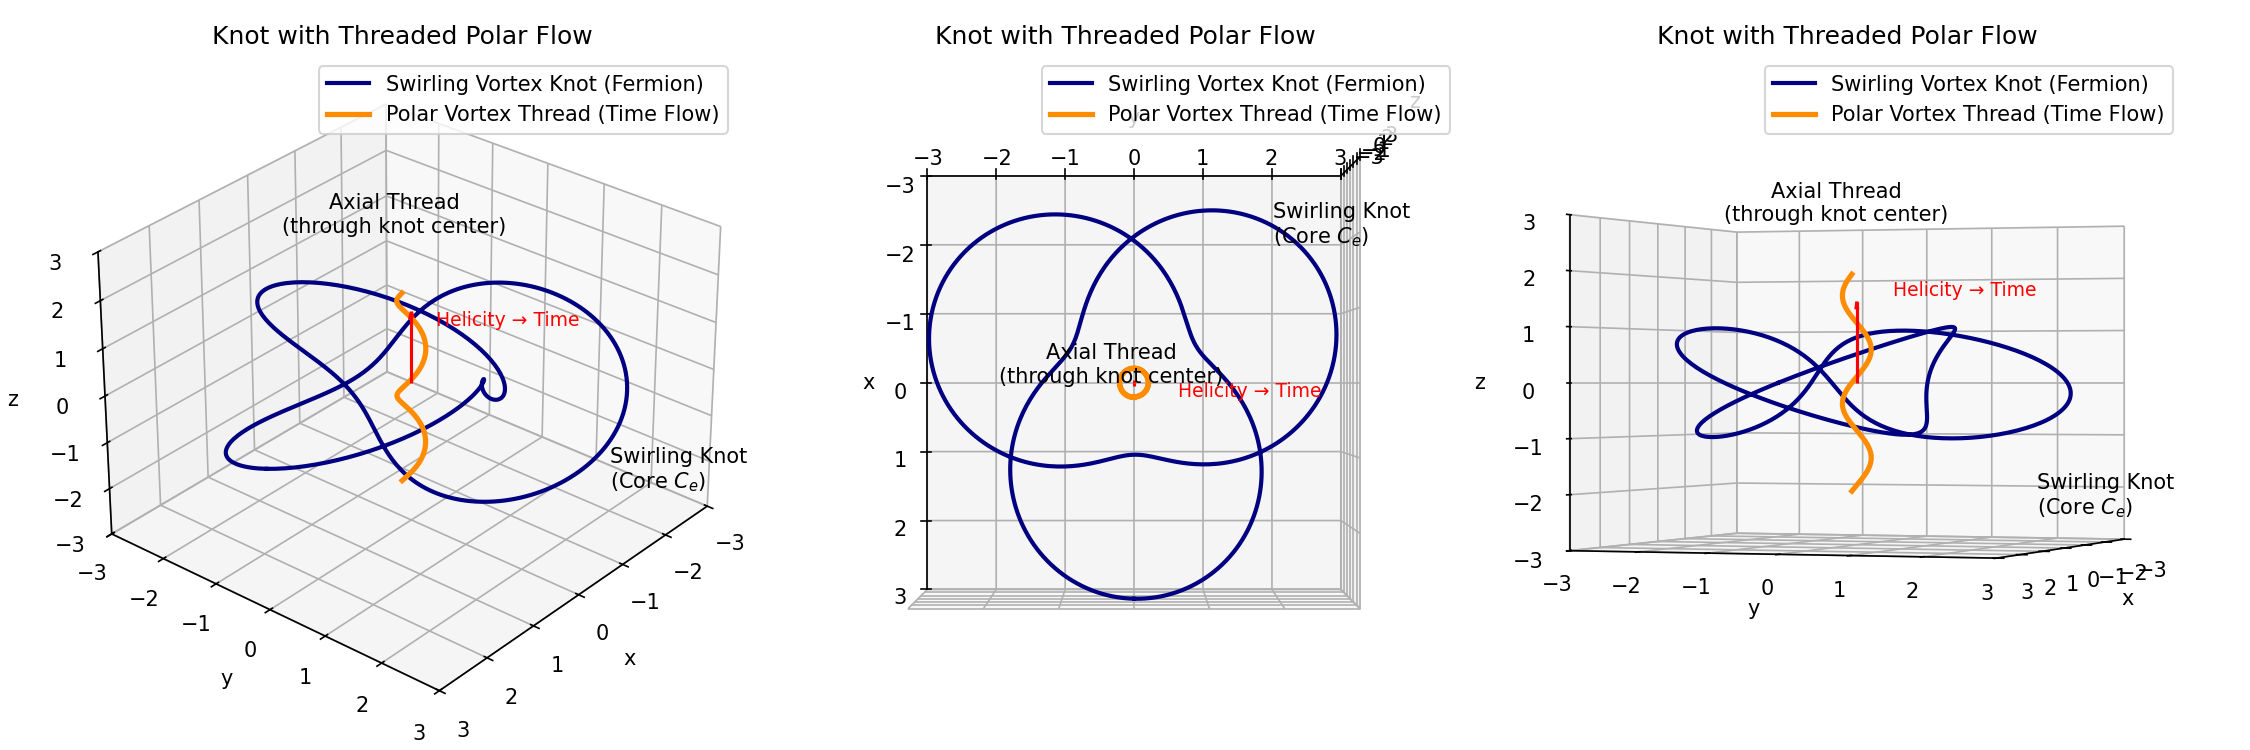
\includegraphics[width=0.85\textwidth]{KnotThreadedPolarFlow}
        \caption{Topological origin of a swirl-thread. The central region of the chiral knot seeds a tightly focused swirl column — a directed vortex axis aligned with the helicity of the knotted flow. This swirl thread forms the basis for local time (vortex phase ticking), mass-energy storage (via internal tension), and interaction capability (swirl-coupling to other knots).}
        \label{fig:knotthreaded}
    \end{figure}

    \subsection{Mass as Swirl Energy Density}

    The swirl thread is not passive — it stores energy. The rotating æther inside this axial tube carries both circulation and strain. From Eq.~(12), the vortex energy is proportional to the integral of the form
    \[
        E \sim \int \rho_{\text{\ae}}^{(\text{energy})} \, \omega^2 \, dV
    \]
    centered on the swirl tube. Since chirality determines swirl orientation and strength, it also determines this energy content. Thus, \textit{mass emerges as a swirl-stored self-energy} proportional to the length and intensity of the axial tube seeded by the knot. In this sense:
    \[
        \text{Mass} \propto \text{Swirl Thread Strength} \propto \text{Knot Chirality} + \text{Topology}
    \]

    \subsection{Swirl-Coupling as Interaction Selector}

    Crucially, these swirl threads define a \textit{directional coupling axis}. Two knots may only interact (bond, scatter, attract) if their swirl vectors are \textit{compatible} — aligned in orientation, handedness, and local phase. This mechanism provides a natural filtering rule:
    \begin{itemize}
        \item Matching swirl threads (e.g., same chirality, phase): attractive coupling, stable binding.
        \item Mismatched swirl (e.g., achiral, opposing helicity): decoupling or expulsion.
    \end{itemize}
    This explains why achiral knots fail to couple and are ejected by the flow: they cannot sustain a consistent swirl-thread in any direction. Instead, their transient swirl attempts cancel out, leading to instability or dispersion — as modeled in Section 6 as candidates for dark energy structures.

    \subsection{Time Flow as Vortex Phase Advancement}

    As shown in Eq.~(17), the internal phase evolution of a chiral knot defines its local time parameter $S(t)$:
    \[
        S(t) = \int \omega(r) \, dt
    \]
    where $\omega(r)$ is the angular frequency of the swirl at a given radius $r$. The swirl-thread defines this $\omega$ field: it seeds the rotation and maintains it. Therefore, the \textit{direction of time}, the \textit{rate of local ticking}, and the \textit{coupling to gravitational curvature} all stem from this axial swirl flow.

    In essence, \textit{chirality seeds time} — it is the source of directed evolution through the æther field, and its persistence is what allows vortex clocks to be defined and synchronized.

    \subsection{Visual Summary}

    Figure~\ref{fig:chiralsummary} illustrates this hierarchy: from a knotted core, a swirl thread extends, storing energy, driving time evolution, and enabling physical coupling. It represents the missing visual link between topology and dynamics — the scaffold of matter, gravity, and gauge interaction in the VAM ontology.

    \begin{figure}[H]
        \centering
        \begin{minipage}{0.25\textwidth}
            \centering
            \includegraphics[width=\textwidth]{knot_5_2_topview}
        \end{minipage}
        \hspace{1em}
        \begin{minipage}{0.25\textwidth}
            \centering
            \includegraphics[width=\textwidth]{knot_6_1_topview}
        \end{minipage}
        \caption{Static knot diagrams used to model up- and down-quark excitations in the VAM baryon framework.\\
        Left: Up-quark \(5_2\) knot. Right: Down-quark \(6_1\) knot.\\
        Swirl thread emergence from knot chirality. Here, a left-handed $T(6,2)$ knot generates an axial swirl field that defines mass, time direction, and interaction potential. Right-handed knots generate mirror-aligned threads (antimatter), while achiral structures lack sustained swirl.}
        \label{fig:chiralsummary}
    \end{figure}



    \subsection*{Outlook}

    This mechanism provides a unifying view: \textit{chirality is not just an invariant — it is the mechanism by which vortex structures gain all the defining properties of particles}: mass, time, and interactions. The swirl-thread formalism clarifies why only some topologies form matter, how time emerges locally in the æther, and why swirl-compatible structures alone participate in binding or scattering.

    In future work, this formalism could be extended:
    \begin{itemize}
        \item To simulate swirl-thread field overlap between knots.
        \item To model decay pathways as swirl instability transitions.
        \item To link quantized swirl helicity with discrete charge.
    \end{itemize}

    It also points to a deeper ontological suggestion: that \textit{time and inertia are emergent, topologically seeded phenomena} — and that the cosmos is stitched together by swirl threads originating in chirality.


\section{Conclusion and Outlook}
    We have presented a LaTeX-written treatise reformulating quantum mechanics and gravity exclusively with the concepts of the Vortex Æther Model. Throughout the paper, every notion – from wavefunctions and spin to curved spacetime and black holes – has been translated into the language of superfluid vorticity, swirl-induced forces, and topological knot invariants. The remarkable outcome is that a single theoretical framework, VAM, can reproduce the content of both quantum field theory and general relativity, using none of their original axioms but rather deriving them from deeper fluid-dynamical principles.

    This exercise underscores several key achievements of VAM:
    \begin{itemize}
        \item It provides \textbf{physical intuition} for quantum phenomena. Rather than abstract Hilbert space and probability amplitudes, we have tangible fluid motions and conserved topological structures. The strange features of quantum theory (duality, uncertainty, entanglement) become less mystical when we see them as properties of a continuous medium with phase coherence and knotted configurations.
        \item It demystifies \textbf{gravity} by eliminating the need for spacetime curvature as a fundamental thing. Instead, gravity’s effects arise from the same substratum that accounts for matter. This aligns with the age-old desire to not have separate realms for geometry and substance: here geometry emerges from substance (æther dynamics) itself.
        \item It \textbf{unifies forces and matter}. Particles are fluid knots, forces are manifestations of the fluid’s response to those knots. Thus, the conceptual gap between matter (fermions) and force fields (bosons) is bridged – both are just patterns in the æther (knotted vs propagating wave patterns). The gauge symmetries are realized as topological symmetries, giving a heuristic why these symmetries exist at all (because of fluid invariances).
        \item It yields quantitative \textbf{derivations of constants} and perhaps addresses fine-tuning issues. If $\hbar$, $G$, particle masses, etc., are calculable from a single set of æther parameters, then the unity of nature’s numbers is explained. Variation of these constants could even be considered if the æther density or core size evolves (tying into cosmology).
    \end{itemize}

    However, the VAM program is in its early stages and faces several challenges and open questions:
    \begin{enumerate}
        \item The \textbf{mathematical rigor} of translating between fluid mechanics and quantum field math needs to be fully established. We have sketched correspondences and cited VAM results, but a full derivation of, say, the path integral for knots reproducing the Standard Model amplitudes is a monumental task.
        \item While VAM avoids introducing \textbf{explicit wavefunctions}, one must be cautious to ensure no contradiction with known quantum theorems (like Bell’s inequality). VAM’s non-local medium might allow violation of Bell locality, but one must check it doesn’t accidentally allow superluminal signalling in practice. The consistent “causal story” of how information flows in the æther while preserving the appearance of relativistic causality needs refinement.
        \item On \textbf{gravity}, VAM thus far has been shown to recover weak-field GR and some strong-field aspects qualitatively. But can it produce gravitational wave dynamics quantitatively identical to GR? Fluid models typically have dispersive or extra modes that might not exactly match GR’s spin-2 massless graviton. This must be studied; perhaps the swirl field’s small oscillations correspond to two transverse modes just like GR’s gravitational waves – if so, VAM could match LIGO results, etc., but if not, discrepancies would arise.
        \item The \textbf{cosmological constant problem} and cosmic inflation are not yet addressed in VAM. Possibly an æther with slight compressibility could mimic dark energy (like a tiny residual pressure). It would be interesting if VAM can naturally explain why the vacuum energy gravitating effect is so small (maybe æther tension self-cancels most of it).
        \item VAM inherits the incompleteness of any emergent theory: we need a \textbf{microphysical underpinning} for the æther itself. Is it made of something? Or is it fundamental? If fundamental, is there an even more primary equation like a preon model or so? VAM currently treats the æther as continuum, but quantum gravity normally implies discreteness at Planck scale. Could the æther be a condensate of more fundamental quanta? One could speculate a connection to other approaches: e.g. maybe VAM’s æther is analogous to the “superfluid vacuum theory” or condensate of hypothetical bosons.
        \item From a \textbf{philosophy of science} perspective, how do we verify a fluid that is mostly intangible? If VAM’s æther only shows itself through subtle quantum and gravitational phenomena, then confirming its existence is indirect. But perhaps one striking lab experiment as mentioned could make it tangible (like seeing time dilation in a superfluid lab experiment would be a clear sign of new physics).
    \end{enumerate}

    The road ahead for VAM research likely involves:
    \begin{itemize}
    \item More sophisticated simulations of knotted æther dynamics to derive effective particle interactions (could computational knot theory meet CFD here).
    \item Designing high-sensitivity experiments in atomic/optical systems to catch small æther effects.
    \item Extending the theory’s mathematical formulation (maybe using knot invariants and algebraic topology to classify multi-itemparticle states, linking with established topological quantum field theory frameworks).
    - Integrating with thermodynamics: if æther flows underlie all, maybe entropy and black hole thermodynamics get new interpretations (perhaps vortex tangle complexity relates to entropy, etc.).
\end{itemize}
    In conclusion, the Vortex Æther Model offers a bold and sweeping vision: that the fabric of reality is a fluid “æther” whose vortices and waves realize everything we observe. This paper has articulated that vision in detail, demonstrating its plausibility by re-deriving known physics within that framework. If VAM (or something akin to it) is correct, the coming years could see a paradigm shift as profound as when quantum mechanics or relativity first emerged – a shift that brings physics back to some classical intuitions (tangible medium) while leaping forward in unification. Whether VAM stands the test of experimental scrutiny remains to be seen. But at the very least, it serves as an enlightening unification exercise, reminding us that our current separate formalisms of quantum and gravity might just be two sides of the same cosmic swirl.





        \begin{thebibliography}{15}

            \bibitem{VAM1}
            O.~Iskandarani, \emph{Time Dilation in a 3D Superfluid Æther Model}, Zenodo (2025).\\
            \url{https://doi.org/10.5281/zenodo.15669795}

            \bibitem{VAM2}
            O.~Iskandarani, \emph{Swirl Clocks and Vorticity-Induced Gravity}, Zenodo (2025).\\
            \url{https://doi.org/10.5281/zenodo.15566336}

            \bibitem{VAM3}
            O.~Iskandarani, \emph{Benchmarking the Vortex Æther Model vs. General Relativity}, Zenodo (2025).\\
            \url{https://doi.org/10.5281/zenodo.15665433}

            \bibitem{VAM4}
            O.~Iskandarani, \emph{Emergent General Relativity from Structured Swirl Dynamics in VAM}, Zenodo (2025).\\
            \url{https://doi.org/10.5281/zenodo.15706539}

            \bibitem{VAM5}
            O.~Iskandarani, \emph{On a Vortex-Based Lagrangian Unification of Gravity and Electromagnetism}, Zenodo (2025).\\
            \url{https://doi.org/10.5281/zenodo.15669904}

            \bibitem{VAM6}
            O.~Iskandarani, \emph{Knotted Gauge Fields and Chiral Vortex Structures}, Zenodo (2025).\\
            \url{https://doi.org/10.5281/zenodo.15669908}

            \bibitem{VAM7}
            O.~Iskandarani, \emph{From Quantum Constants to Galactic Swirl}, Zenodo (2025).\\
            \url{https://doi.org/10.5281/zenodo.15772855}

            \bibitem{VAM8}
            O.~Iskandarani, \emph{The Vortex Æther Model: Master Formulation}, Zenodo (2025).\\
            \url{https://doi.org/10.5281/zenodo.15772859}

            \bibitem{VAM9}
            O.~Iskandarani, \emph{Milky Way as a Chiral Swirl-Knot Network}, Zenodo (2025).\\
            \url{https://doi.org/10.5281/zenodo.15772861}

            \bibitem{VAM10}
            O.~Iskandarani, \emph{Swirl-Induced Curvature as the Mechanism of Gravitation}, Zenodo (2025).\\
            \url{https://doi.org/10.5281/zenodo.15669892}

            \bibitem{VAM11}
            O.~Iskandarani, \emph{Master Equation for Particle Masses}, Zenodo (2025).\\
            \url{https://doi.org/10.5281/zenodo.15706536}

            \bibitem{VAM12}
            O.~Iskandarani, \emph{Fractal Swirl: Nested Structure of the Vortex Æther}, Zenodo (2025).\\
            \url{https://doi.org/10.5281/zenodo.15772860}

            \bibitem{VAM13}
            O.~Iskandarani, \emph{Beyond Spacetime: A Fluid-Dynamic Theory of Gravity and Time from Vorticity}, Zenodo (2025).\\
            \url{https://doi.org/10.5281/zenodo.15706547}

            \bibitem{VAM14}
            O.~Iskandarani, \emph{Topological \& Fluid-Dynamic Lagrangian in the Vortex Æther Model}, Zenodo (2025).\\
            \url{https://doi.org/10.5281/zenodo.15772858}

            \bibitem{irvine2013-knots}
            W.~T.~M. Irvine and D.~Bouwmeester, \emph{Linked and knotted beams of light},\\
            \emph{Nature Physics} \textbf{9}, 790–795 (2013).\\
            \url{https://doi.org/10.1038/nphys2483}

        \end{thebibliography}


\end{document}
